% !Mode:: "TeX:UTF-8"
\chapter{Описание предлагаемых методов и моделей}

\section{Описание предлагаемого подхода генерации тестовых программ}\label{sec:approach}
Предлагаемый подход целенаправленного построения тестовых программ состоит из следующих шагов (их подробное описание будет дано ниже):
\begin{enumerate}
    \item чтение документации по архитектуре;
    \item формализация архитектуры;
    \item выделение и формализация тестовых ситуаций (в виде тестовых шаблонов);
    \item построение системы ограничений для каждой тестовой ситуации;
    \item решение системы ограничений;
    \item конструирование текста тестовой программы на основе результатов решения системы ограничений.
\end{enumerate}

В рамках технологий разработки микропроцессоров и архитектур микропроцессоров кроме исходных текстов моделей микропроцессоров готовится документация с описанием системы инструкций. Этот документ становится основой для генерации тестов. Документ должен обладать достаточным уровнем детальности, чтобы в нем были представлены все \emph{варианты исполнения} всех инструкций (ветви функциональности). Сперва разработчики тестов <<размечают>> описания инструкций --- выделяют варианты исполнения инструкций. Тестовая программа представляет собой последовательность зависимых инструкций. Каждая инструкций исполняется согласно своему варианту исполнения, операнды инструкций зависят друг от друга так, что все вместе эти инструкции создают особую ситуацию в работе микропроцессора. Зафиксировав последовательность инструкций, их варианты исполнения и то, как зависят операнды одних инструкций от других, будет формализована и ситуация в работе микропроцессора --- \emph{тестовая ситуация}. Разработчик тестов обладает знанием того, какие нужны тестовые ситуации. Он формализует последовательность инструкций, операнды инструкций и варианты инструкций в виде \emph{тестовых шаблонов}. С достаточной степенью общности можно сказать, что шаблон задает набор параметров и набор отношений на их значения. Такими параметрами являются начальные значения регистров, флагов, хранящиеся данные в устройствах подсистемы управления памяти (например, в кэш-памяти). Эти отношения разработчик теста должен выразить с использованием техники ограничений. Затем с использованием известных методов разрешения ограничений разработчик тестов находит значения параметров, для которых ограничения выполнены. На заключительном этапе по вычисленным значениям параметров строится последовательность инструкций, соответствующая тестовому шаблону. Эта последовательность содержит дополнительные инструкции для инициализации микропроцессора (среди параметров присутствуют параметры, ответственные за помещение микропроцессора в то состояние, из которого правильно реализованные инструкции будут исполняться согласно тестовому шаблону).

В рамках подхода задействованы различные специальные модели и методы (см. рисунок~\ref{fig:process}). Этапы подхода на рисунке помещены в прямоугольники с закругленными краями, их названия выделены полужирным шрифтом. Остальные прямоугольники означают различные модели, данные, документы, вовлекаемые в процесс построения тестов. От данных, являющихся исходными для этапов, нарисованы стрелки к этапам. К данным, являющимся выходными для этапов, нарисованы стрелки от этапов. Имеется одна развилка по результатам решения составленной системы ограничений --- система ограничений либо совместна, либо несовместна. В последнем случае делается заключение о том, что для данного шаблона для данного микропроцессора не существует ни одной соответствующей ему тестовой программы.

Везде речь идет о тестировании, нацеленном на подсистему управления памяти, хотя подход без изменений применим и для тестирования, нацеленного на некоторые другие подситемы микропроцессоров, например. на арифметическую подсисетму. Но для подсистем управления памяти разработаны особые новые методы моделирования и построения ограничений с учетом возможностей существующих инструментов для автоматического разрешения ограничений.

%\begin{figure}[h] \center
%  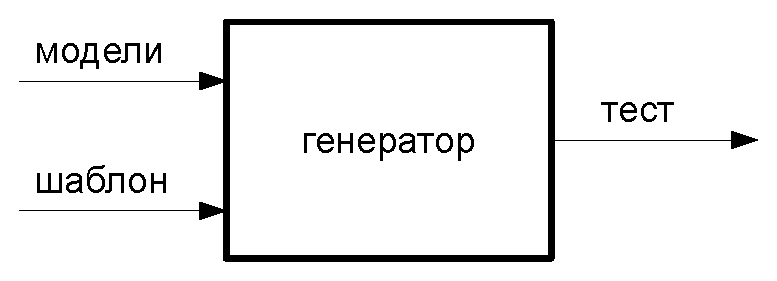
\includegraphics[width=0.5\textwidth]{2.theor/common_view}\\
%  \caption{Схема автоматизации подхода}\label{fig:common_view}
%\end{figure}
%
%Схема автоматизации подхода изображена на рисунке~\ref{fig:common_view}. Она предполагает использование автоматического \emph{генератора} тестов, которому на вход подаются различные модели --- результат формализации архитектуры --- и шаблоны --- результат этапа выделения тестовых ситуаций. Внутри генератора находятся последние шаги подхода ---- генератор ограничений, решатель ограничений и конструктор текстов тестовых программ. Этапы по подготовке входных данных генератора и самого генератора собраны в схеме на рисунке~\ref{fig:process}. Действия, которые надо выполнить вручную, помещены в прямоугольники с закругленными краями. Данные помещены в прямоугольники. Программные компоненты помещены в параллелограммы~\cite{my_lomonosov_2009, my_miet_2009}.
%\begin{enumerate}
%  \item чтение документации по архитектуре;
%  \item формализация архитектуры;
%  \item выделение интересных для тестирования ситуаций;
%  \item подготовка конструктора инициализирующей программы;
%  \item запуск генератора для каждой ситуации.
%\end{enumerate}


\begin{figure}[p] \center
  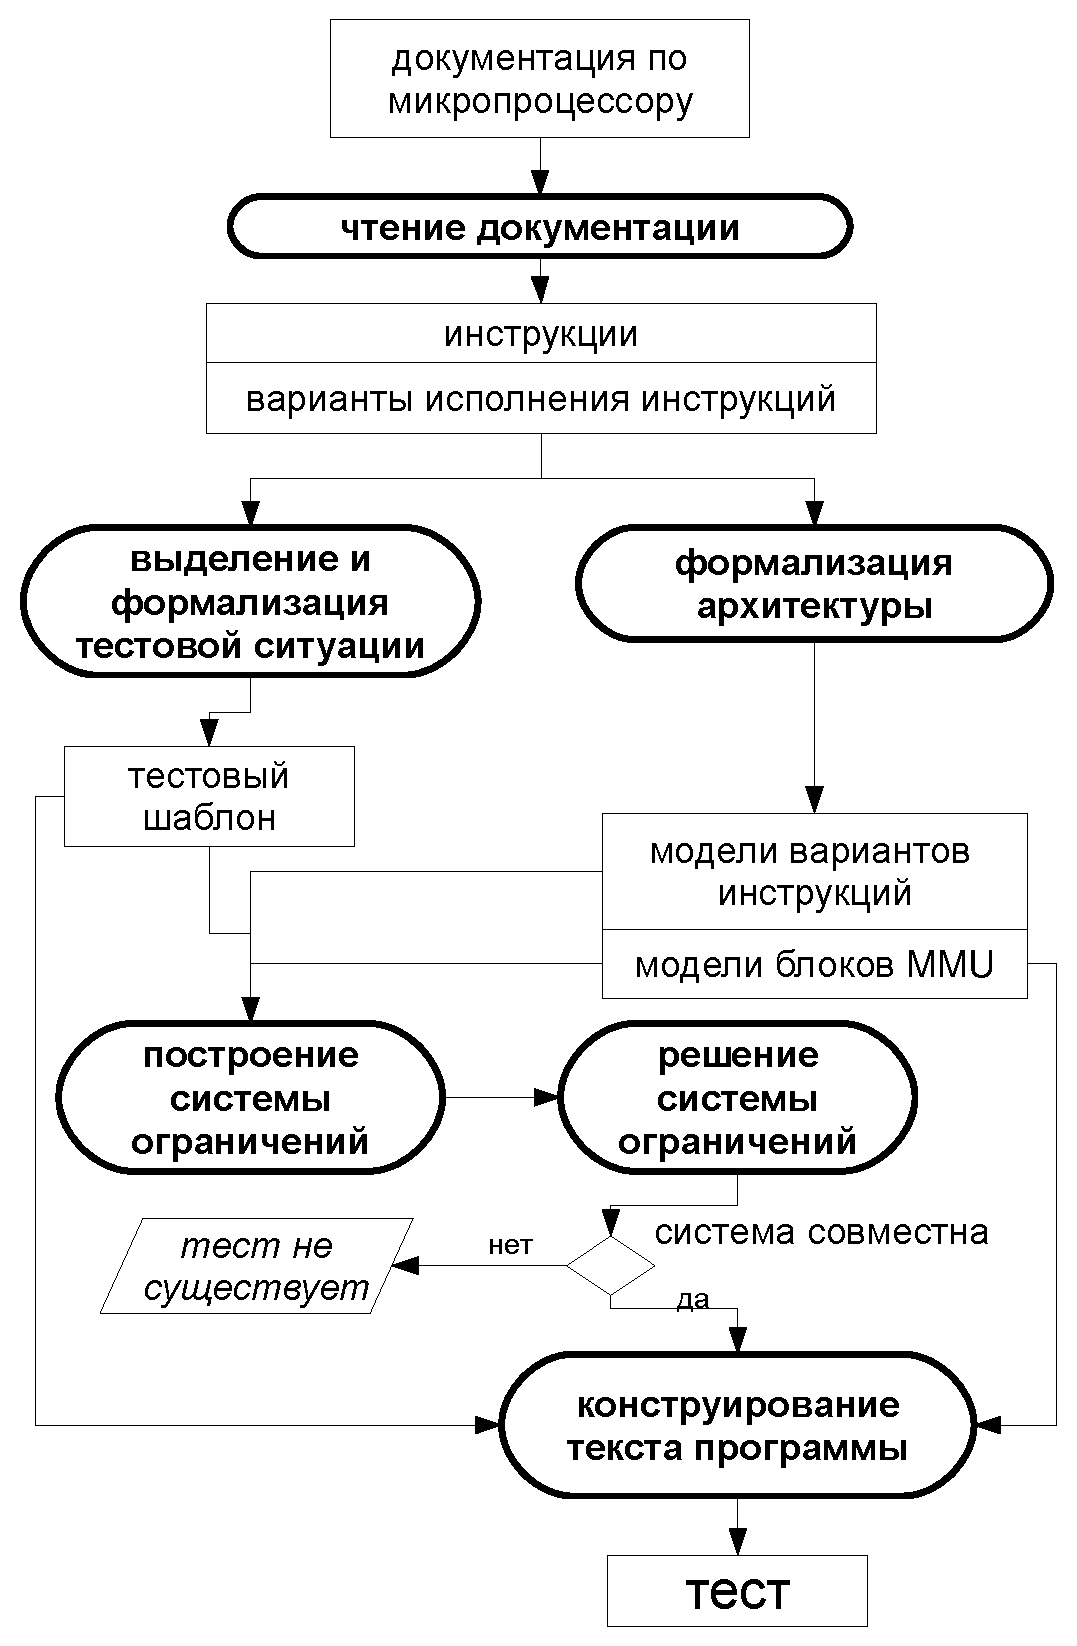
\includegraphics[width=0.8\textwidth]{2.theor/process_manual}\\
  \caption{Подход генерации тестовых программ}\label{fig:process}
\end{figure}

Далее более подробно будут описаны отдельные этапы предлагаемого метода.

\subsubsection{Чтение документации}%\label{sec:reading_stage}

<<Документация по архитектуре>> --- это документ, описывающий семантику инструкций микропроцессора и некоторые структурные особенности микропроцессора (кэш-память, различные буферы, и др).
В рамках данного этапа следует читать эту документацию и сделать следующее:
\begin{enumerate}
  \item выделить инструкции, их формат (какие возможны аргументы -- регистры, непосредственные значения и т.п.);
  \item выделить варианты исполнения инструкций (<<разметить>>, обычно один вариант исполнения описывается в виде последовательности более простых действий), каждому варианту исполнения присвоить идентификатор (метку); зафиксировать последовательность действий и условий в рамках этого варианта;
  \item определить для каждого варианта исполнения устройства микропроцессора, в которые происходят в нем обращения (кэш-память некоторых уровней, буфер трансляции адресов и т.п.).
\end{enumerate}

Например, по результатам чтения документации по инструкции обращения в память могут быть выделены следующие варианты этой инструкции:
\begin{itemize}
    \item возникновение исключения по причине невыровненного адреса;
    \item обращение в оперативную память без кэш-памяти;
    \item обращение в оперативную память с предварительным обращением в кэш-память;
    \item при обращении в кэш-память происходит кэш-промах.
\end{itemize}

%На данном этапе описание варианта исполнения этой инструкции может быть таким: 1) вычисляется виртуальный адрес --- сумма аргументов, 2) если <<виртуальный адрес отображаемый>>, вычисляется номер виртуальной страницы, для нее в TLB ищется соответствующая страница физической памяти (<<идет обращение в TLB>>), иначе вычисляется физический адрес как битовая подстрока виртуального адреса и т.д.

\subsubsection{Выбор и формализация тестовых ситуаций}%\label{sec:template_stage}

В рамках этого этапа тестовые ситуации должны быть формализованы в виде тестовых шаблонов. Тестовый шаблон состоит из заголовка и тела шаблона. Заголовок состоит из определений операндов инструкций шаблона: регистров и констант-непосредственных значений. Определение включает в себя имя и битовую длину. Например, определение 64-битного регистра \texttt{r1} и 16-битовой константы \texttt{c} выглядит так:
\begin{verbatim}
register r1 : 64;
const c : 16;
\end{verbatim}
Тело тестового шаблона состоит из последовательности помеченных инструкций. Помеченная инструкция состоит из названия, операндов (их имена указаны в заголовке шаблона) и варианта исполнения инструкции (идентификатора-метки, которая была присвоена этому варианту исполнения при чтении документации). Например:

\begin{figure}[h]
{ \tt
register x: 64; register y:64; const c: 16;\\
LW x, y, c @ l1Hit }
\caption{Пример тестового шаблона}\label{test_template_exmp1}
\end{figure}

%\begin{figure}[h]
%\quad\parbox{0.5\textwidth}{ \tt
%LW x, y, c @ l1Hit } \parbox{0.3\textwidth}{ \tt
%XOR y, y, y\\
%SW x, y, 0x0\\
%LW x, y, 0x0\\}
%\caption{Тестовый шаблон (слева) и один из возможных тестов для него
%(справа)}\label{test_template_exmp1}
%\end{figure}

Согласно сделанному в главе 1 обзору, имеются работы, в которых предлагаются методы автоматического построения тестовых шаблонов.

\subsubsection{Формализация архитектуры}

Этот этап предполагает моделирование устройств подсистемы управления памяти и вариантов исполнения инструкций (формализация <<идентификаторов>> из тестовых шаблонов, обозначающих варианты исполнения инструкций). Детальное описание того, что из себя представляют эти модели, будет дано в разделе~\ref{sec:state_model_section}.

Моделирование устройства подсистемы управления памяти происходит в терминах расширенных конечных автоматов. Модель состояния устройства формализует хранящиеся в устройстве данные (например, кэш-строки в кэш-памяти). Переходы в автомате помечены операциями обращения в это устройство: попадания и промахи. В рамках этапа формализации архитектуры следует задать ряд структурных и функциональных характеристик для каждого моделируемого устройства подсистемы управления памяти.

Модели вариантов исполнения инструкций детализируют и формализуют функциональность инструкции. Формализованное описание варианта исполнения инструкции представляет из себя последовательность операторов специального языка (этот язык и механизмы, которые он предоставляет, будут описаны в разделе~\ref{sec:state_model_section}). Язык для описания вариантов инструкций приближен к тому, как в большинстве случаев описываются инструкции в документации, приближен к псевдокоду, использующемуся в документации. Это упрощает этап формализации инструкций. В разделе~\ref{sec:state_model_section} будут приведены примеры моделей и процесса их построения.

\subsubsection{Построение и решение системы ограничений для тестового шаблона}

Тестовый шаблон задает не только последовательность инструкций и их операнды, но и множество допустимых состояний микропроцессора перед первой инструкцией шаблона. Состояние считается допустимым, если исполненные из него инструкции будут именно в тех вариантах, которые указаны в шаблоне. Наступление нужного варианта зависит от того, какие значения в регистрах, какие установлены флаги, какие области памяти помещены в кэш-память, а какие нет. С достаточной степенью общности такое состояние представимо множеством зависимых параметров. Нас интересуют такие значения параметров, которые соответствуют вариантам исполнения инструкций. Поскольку варианты исполнения инструкций были формализованы на предыдущем этапе, то возможно алгоритмическое выделение нужных параметров и того, Как значения одних параметров должны зависеть от значений других параметров. Техника ограничений позволяет выразить отношения значений параметров и алгоритмически отыскать их значения, которые удовлетворяют отношениям.

Этап выполняется в два шага
\begin{itemize}
  \item выделить параметры;
  \item выделить ограничения на эти параметры.
\end{itemize}

В разделе~\ref{sec:constraints_generation_section} будет описано, как надо выполнять эти шаги. Параметры выбираются, так, чтобы задать все необходимые для инициализации устройств данные и значения в регистрах (начальные и промежуточные). Ограничения составляются путем трансляции описаний вариантов исполнения инструкций оператор за оператором.

Составленная система ограничений исследуется на совместность. Возможны 2 случая: построенная система ограничнеий несовместна или система ограничений совместна. Если она совместна, то она решается и получаются значения параметров. Если система ограничений несовместна, то (как будет следовать из теорем о корректности и полноте) для данного тестового шаблона не может существовать ни одной тестовой программы.

\subsubsection{Конструирование текста тестовой программы}

Заключительным этапом является составление текста тестовой программы.  К этому моменту известно, что для тестового шаблона существует тестовая программа и вычислены подходящие значения параметров. Теперь надо построить последовательность инструкций, инициализирующих микропроцессор и выполняющих заданную тестовую ситуацию. Построение тестовой программы проводится следующим образом:
\begin{enumerate}
  \item построение \emph{инициализирующей подпрограммы};
        \begin{enumerate}
          \item инициализация каждого необходимого регистра (среди параметров есть начальное значени ерегистра; нужно составить 1 инструкцию, помещающую значение этого параметра е регистр);
          \item инициализация каждого необходимого устройства подсистемы управления памяти (среди параметров есть те, что относятся к инициализации этого устройства --- из них надо составить последовательность инструкций, подробнее этот момент описан в разделах~\ref{sec:constraints_generation_section} и \ref{sec:L1L2_initialization});
        \end{enumerate}
  \item построение инструкций тестовой ситуации (инструкции тела тестового шаблона, в которых на место констант-непосредственных значений подставлены вычисленные значения соответствующих им параметров).
\end{enumerate}

%Конкретный формат инструкций обращения к памяти, работающий с заданным блоком MMU, определяется архитектурой микропроцессора и обычно описывается в документации. Например, в архитектуре MIPS64~\cite{mips64III} зафиксирована семантика диапазонов виртуальных адресов: обращение по некоторым виртуальным адресам приводит к исключительной ситуации \texttt{AddressError}, по некоторым --- обращение в память проводится без буфера трансляции адресов (TLB), по некоторым --- с использованием TLB, по некоторым --- обращение в память проводится без кэш-памяти и т.д. Зная параметры отдельной инструкции, инициализирующей блок MMU, и зная эту семантику, надо составить аргументы инструкции и, возможно, построить инструкции для смены режима работы микропроцессора.

На рисунке~\ref{fig:blocks_init_examples} приведены части программ, инициализирующих MIPS64-совместимые микропроцессоры. В левой половине подготавливается и записывается одна строка TLB . Для этого подготавливаются системные регистры \$0, \$2, \$3, \$10. В конце идет инструкция \texttt{tlbwi}, которая записывает строку в TLB на основе значений в регистрах \$0, \$2, \$3, \$10. В правой половине рисунка~\ref{fig:blocks_init_examples} приведена подпрограмма для подготовки и записи одной строки кэш-памяти первого уровня L1. Для этого первые инструкции помещают в регистр \texttt{r13} виртуальный адрес, а расположенная последней инструкция \texttt{sd} осуществляет обращение в память по этому адресу. В этом обращении изменяется состояние кэш-памяти L1: в нее записывается нужная строка. Все эти инструкции строятся на этапе конструирования текста тестовой программы, зная строки (т.е. зная значения параметров-составляющих строки). Какими именно инструкциями нужно воспользоваться, чтобы поместить строки в определенные устройства подсистемы управления памяти, зависит от документации. На этом этапе надо, проанализировав документацию, извлечь из нее или составить самостоятельно соответствующие подпрограммы для работы с нужными устройствами и использовать их для конструирования текстов тестовых программ.  инструкцией sd (store doubleword).

\begin{figure}[h] \centering
\parbox{0.4\textwidth}{
строка TLB:\\
{\small \tt
    ori r13, r0, 0x0\\
    mtc0 r13, \$0\\
    lui r13, 0x0\\
    dmtc0 r13, \$10\\
    ori r13, r0, 0x1f\\
    mtc0 r13, \$2\\
    ori r13, r0, 0x1f\\
    mtc0 r13, \$3\\
    tlbwi\\}
} \qquad
\parbox{0.4\textwidth}{
строка L1:\\
{\small \tt
    ori r13, r0, 0x9800\\
    dsll r13, r13, 16\\
    dsll r13, r13, 16\\
    dsll r13, r13, 16\\
    sd r13, 0(r13)\\}
} \caption{Примеры частей инициализирующих подпрограмм для различных устройств}\label{fig:blocks_init_examples}
\end{figure}


%Этот этап (как следует из его названия) предполагает подготовку соответствующего конструктора. Тестовый шаблон еще не может быть тестом, поскольку в нем не заданы значения аргументов инструкций и не актуализировано начальное состояние микропроцессора (предполагается, что оно должно быть \emph{таким}, чтобы инструкции выполнялись заданным образом).
%
%Поэтому после того, как подготовлен тестовый шаблон, модели блоков MMU и формализованы описания вариантов исполнения инструкций, в работу включаются компоненты, осуществляющие построение недостающих данных и актуализацию начального состояния микропроцессора. Например, для шаблона на рисунке~\ref{test_template_exmp1} было выбрано значение переменной <<c>> (оно равно 0) и актуализировано начальное состояние в виде последовательности инструкций \texttt{XOR y, y, y} и \texttt{SW x, y, 0x0}.
%
%В рассматриваемом методе предлагается актуализировать начальное состояние в виде последовательности инструкций (которые образуют \emph{инициализирующую программу}). Поскольку речь идет о тестировании модулей управления памяти, то эти последовательности инструкций должны затрагивать блоки микропроцессора, отвечающие работе с памятью. Специальные последовательности таких обращений должны подготовить эти блоки к требуемым вариантам исполнения в тестовом шаблоне. Для каждого блока будет своя такая последовательность. И еще одна последовательность для инициализации регистров общего назначения. Инициализирующая программа --- это обычная программа на языке ассемблера, но эта программа должна давать специфический эффект -- инициализировать блоки микропроцессора.
%
%Построение инициализирующей программы было разделено на ряд этапов:
%\begin{enumerate}
%  \item построение \emph{ограничений} (constraint'ов) по шаблону, модели состояния и описаниям инструкций; речь идет о построении ограничений на \emph{данные}; в эти данные входят значения переменных в описаниях инструкций, атрибуты инструкций инициализирующих инструкций (адреса, к которым производятся обращения, вид обращения и т.п.);
%  \item разрешение ограничений (вычисление данных);
%  \item конструирование инициализирующей программы на основе вычисленных данных; их надо облечь в вид инструкций тестируемой архитектуры --- этот этап и выполняет конструктор инициализирующих программ; например, для каждой будущей инструкции выбрать регистры-аргументы, вычислить на основе переданных атрибутов инструкции значения аргументов, сгенерировать инструкции, обеспечивающие значения аргументов, и саму инструкцию, для которой это всё делалось.
%\end{enumerate}
%
%Иными словами, для построения данных (значений переменных, атрибутов инструкций инициализирующей программы) используется аппарат ограничений (Constraint Satisfaction Problem)~\cite{CSP}. Известно, что время разрешения ограничений сильно зависит от самих ограничений~\cite{isaac05balanced}. Одна и та же задача представима в виде разных наборов ограничений: одни быстрее разрешаются, другие долго. Ограничения для инструкций работы с памятью, видимо, должны учитывать состояния (содержимое!) различных блоков, размеры которых (количество данных) выражается переменными в количестве $10^4-10^5$ штук. Тем самым ограничения надо строить неким особым способом, чтобы справиться с этим количеством зависимых переменных. В разделе~\ref{sec:constraints_generation_section} подробно разбираются предлагаемые в диссертации методы построения ограничений. Важный вопрос --- является ли метод построения ограничений полным, т.е. дает ли метод построения ограничений гарантию того, что если решатель обнаружил несовместность ограничений, то для такого шаблона не существует теста. В разделе~\ref{sec:constraints_generation_section} предлагается полный метод, его полнота доказана в приложении~\ref{sec:proofs}.
%
%Существенно, что в качестве решателей ограничений в описываемом методе достаточно использовать широко используемые решатели (например, Z3~\cite{Z3}). Это выгодно отличает эту работу от аналогичных~\cite{GenesysPro}, где приходится использовать специальные методы не только построения, но и разрешения ограничений, дабы иметь возможность описывать более сложные инструкции.
%
%При написании конструктора достаточно знания того, как загрузить заданные значения в регистры, как обратиться по заданным адресам в память, загрузить в память заданные значения. Это знание получается в результате знакомства с документацией по архитектуре микропроцессора. Кроме того, нужно использовать знание модели состояния, поскольку последовательности данных об инструкциях инициализирующей программы определяются для ограничений (constraint'ов) в терминах этой модели.

\section{Моделирование устройств подсистемы \\управления памяти и вариантов исполнения инструкций}\label{sec:state_model_section}

Устройства подсистемы управления памяти (кэш-память, таблицы страниц и т.п.) предлагается моделировать в виде расширенных конечных автоматов с заданным набором операций. Моделью состояния такого автомата предлагается последовательность ассоциативных массивов (далее эта последовательность будет называться \emph{таблицей}, а отдельный ассоциативный массив --- \emph{регионом}). Каждый регион состоит из \emph{строк}, каждая строка состоит из набора \emph{полей} (поименованных битовых строк), поля делятся на \emph{поля ключа} и \emph{поля данных}. Поля ключа задают ключи в ассоциативном массиве, поля данных --- значения. Все регионы одной таблицы состоят из одинакового количества строк. Все строки одной таблицы имеют одну и ту же структуру полей. С точки зрения вытеснения все регионы должны себя вести независимо. Один регион составляют строки, среди которых при вытеснении определяется вытесняемая строка. Все регисоны пронумерованы последовательно, начиная с нуля. Количество регионов должно быть степенью двойки.\\

\begin{figure}[h] \center
  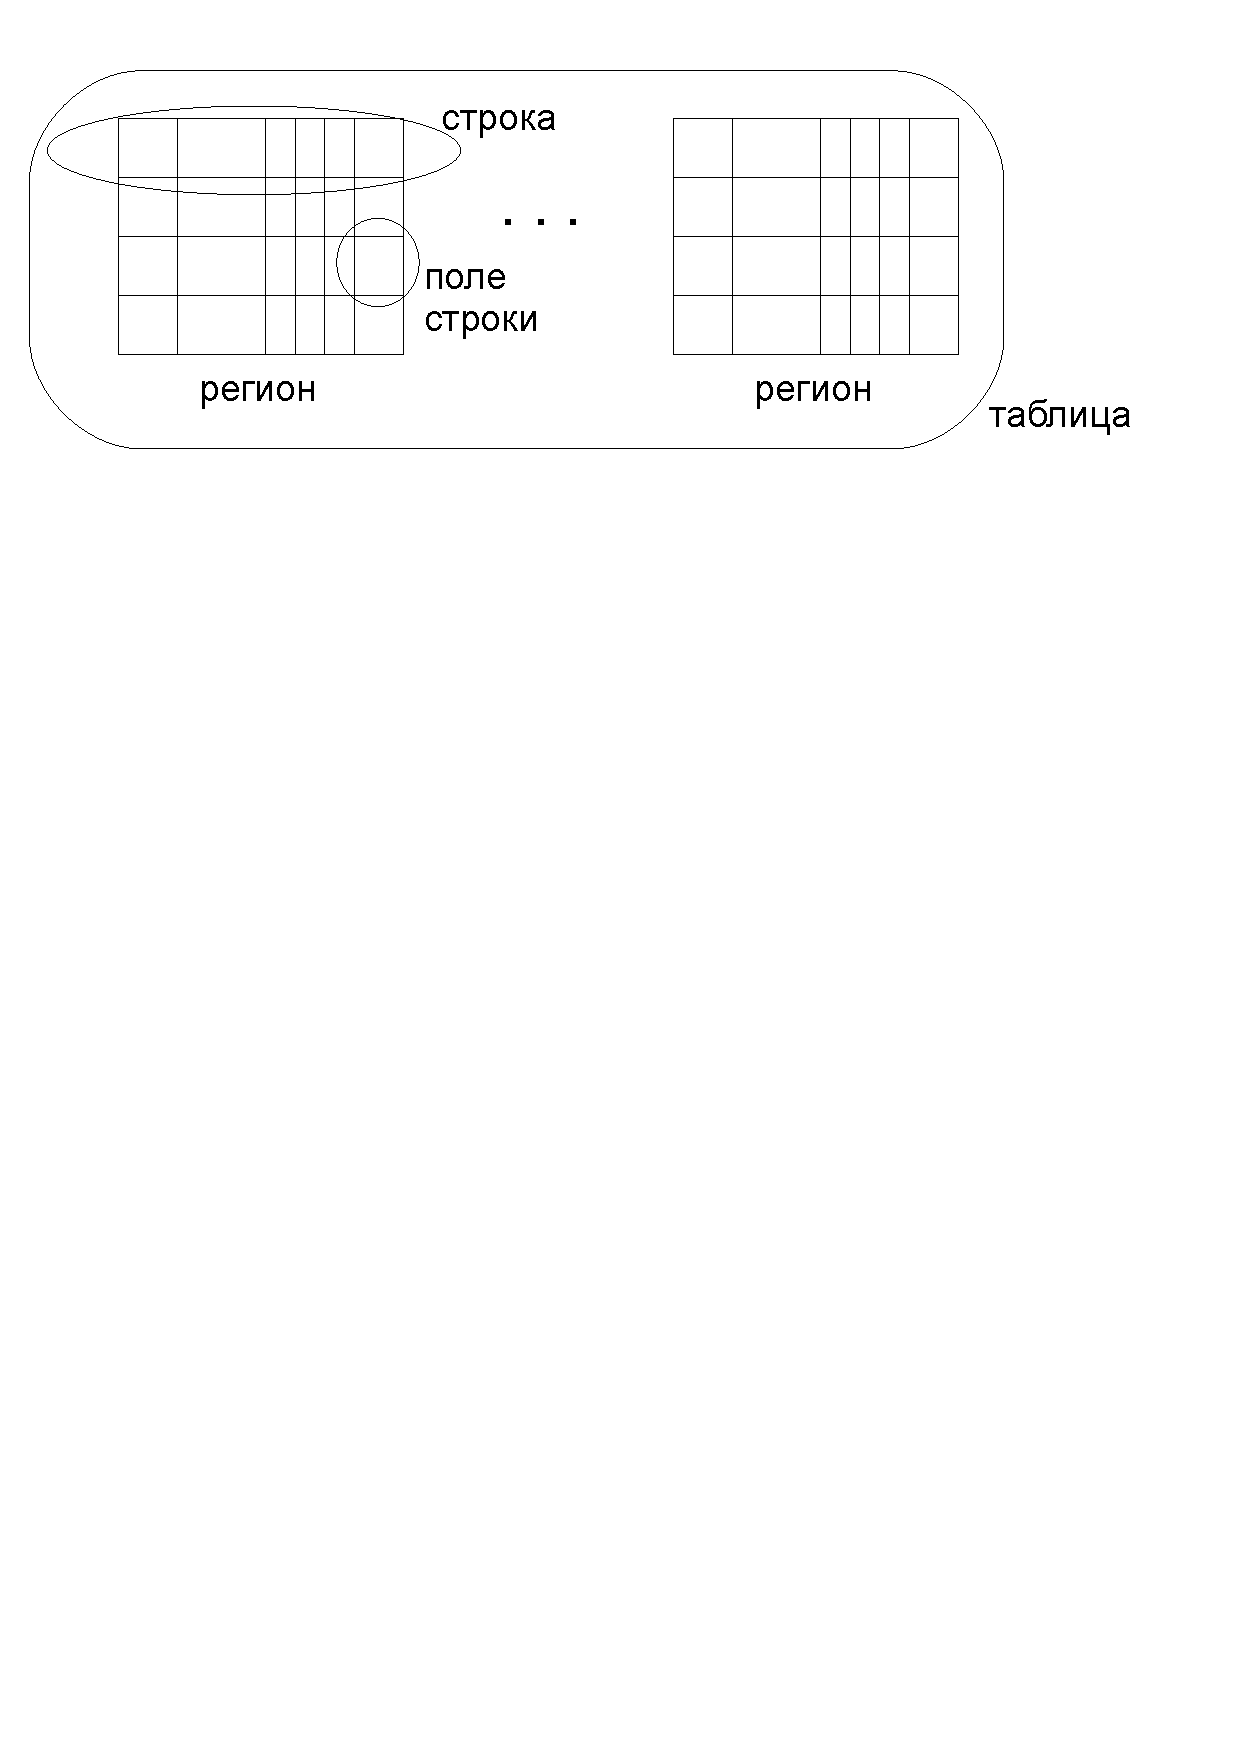
\includegraphics[width=0.8\textwidth]{2.theor/table}\\
  \caption{Таблица}\label{table_picture}
\end{figure}

Рассуждая для кэш-памяти (ее структура описана в разделе~\ref{section:cache}), строками будут кэш-строки с тегами адресов. Регион будут составлять кэш-строки из всех секций, расположенные по одному и тому же индексу. Количество строк в регионе  равно количеству секций, т.е. ассоциативности кэш-памяти $w$. Количество регионов равно количеству кэш-строк в секции.

Буфер трансляции (TLB) в микропроцессорах архитектуры MIPS64~\cite{mips64III} состоит из строк, каждая строка содержит ряд полей, в том числе половину номера виртуальной страницы $v$, номер физического кадра, соответствующего виртуальной странице с номером $2v$, и номер физического кадра, соответствующего виртуальной странице с номером $2v+1$. Обращение в буфер происходит по некоторому виртуальному адресу. Если его половина присутствует в одной из строк TLB, то вычисляется физический адрес на основе одного из номеров физических кадров той же строки. Эту ситуацию будем считать <<попаданием>>. Если его половине не присутствует ни в одной из строк TLB, ситуацию будем считать <<промахом>>. При этом одна из строк будет вытеснена и заменена другой (это делается программно так же, как показано на рисунке~\ref{fig:blocks_init_examples}. Поэтому буфер трансляции адресов в микропроцессорах архитектуры
MIPS64 моделируется таблицей из одного региона, каждая его строка состоит из полей \texttt{r}, \texttt{vpn/2}, \texttt{g}, \texttt{asid}, \texttt{pfn}$_0$, \texttt{CCA}$_0$, \texttt{v}$_0$, \texttt{pfn}$_1$, \texttt{CCA}$_1$, \texttt{valid}$_1$ и других.

Упор на вытеснение сделан неслучайно: как показано в разделе~\ref{section:cache}, ряд важных ошибок связан именно с некорректной реализацией вытеснения. Предлагаемые здесь модели составляются для устройств подсистемы управления памяти, обладающих вытеснением. Это кэш-память всех уровней, таблицы трансляции адресов. Таким же образом можно смоделировать и оперативную память: строка такой таблицы содержит физический адрес и данные по нему, каждый регион состоит из одной строки.

В модели устройства определены следующие операции:
\begin{itemize}
    \item успешного обращения;
    \item успешного обращения с изменением;
    \item неуспешного обращения с замещением.
\end{itemize}

На входе операции успешного обращения --- выражение, задающие ключ, и выражение, задающее номер региона таблицы. Операция определена на тех входных данных и состоянии модели устройства, при которых в соответствующем ассоциативном массиве есть строка, поля ключей которой \emph{соответствуют} аргументу-ключу этой операции. Операция возвращает поля данных соответствующей аргументу-ключу строки. Операция успешного обращения с изменением отличается от операции успешного обращения дополнительным аргументом --- полями данных, которые нужно заменить в строке, соответствующей аргументу-ключу. На входе операции  неуспешного обращения с замещением 3 аргумента: выражение, задающие ключ, выражение, задающее номер региона, и выражения для полей данных строки. Операция определена на тех входных данных и состоянии модели, при которых в соответствующем регионе нет строки, поля ключей которой \emph{соответствуют} аргументу-ключу этой операции. Эффект операции заключается в замене полей данных одной из строк в регионе, номер которого был передан в качестве одного из аргументов операции, на переданные операции поля данных. Выбор строки для замены определяется на основе стратегии вытеснения так же, как это делается в устройствах подсистемы управления памяти (например, в кэш-памяти).

На строках таблицы определено отношение одинакового ключа. Две строки находятся в этом отношении, если существует ключ-аргумент операции обращения в таблицу, которому соответствуют эти обе строки. Отношение задается только на полях ключа. В одном регионе не должно быть двух строк, находящихся в отношении одинакового ключа (поскольку регион --- это ассоциативный массив).

Экземпляр таблицы задается значениями следующего ряда параметров (эти значения составляют \emph{описание таблицы}):
\begin{itemize}
    \item название таблицы;
    \item line --- поля строк (для каждого поля указывается название, битовая длина, поле
ли это ключа или поле данных);
    \item regionbits --- битовая длина номера региона (двоичный логарифм количества регионов);
    \item policy --- стратегия вытеснения; возможные значения: <<none>> (означает отсутствие вытеснения при неуспешном обращении), <<\LRU>>, <<\FIFO>>, <<\PseudoLRU>> и др;
    \item lines --- количество строк в регионе;
    \item keyMatch --- предикат от аргументов операции обращения и полей ключа строки; он истинен в том и только том случае, когда строка соответствует аргументам операции (тегам физического адреса, номерам виртуальных страниц и т.п.).
\end{itemize}

Описание модели уже упомянутого буфера трансляции адресов микропроцессоров архитектуры
MIPS64 выглядит следующим образом:
\begin{verbatim}
table TLB
{
    line(   r:2:key, vpnd2:28:key, g:1:key, asid:4:key,
            pfn0:24:data, cca0:3:data, valid0:1:data,
            pfn1:24:data, cca1:3:data, valid1:1;data );
    regionbits = 0;
    policy = none;
    lines = 48;
    keyMatch(r:2, vpnd2:28) { .... };
}
\end{verbatim}

Предикат keyMatch будет приведен чуть позже, когда будет описан для этого язык.

Теперь переходим к языку описания формализованных вариантов исполнения инструкций (или просто, языку описания инструкций). На предыдущих этапах вариант исполнения задавался в виде последовательности неформализованных действий. Формализованное описание инструкции повторяет эту последовательность, внося ряд уточнений. В документации по микропроцессору вариант исполнения инструкции описывается на псевдокоде в виде последовательности преобразований-операторов, причем большая их часть --- это операторы над битовыми строками (например, значениями регистров, виртуальных адресов, физических адресов). Предлагаемое в диссертации описание следует этому же принципу: это последовательность операторов над битовыми строками и двух дополнительных операторов, специфичных блокам подсистемы управления памяти.

Грамматика языка описания вариантов инструкции в виде расширенной формы Бэкуса-Наура приведена в приложении~\ref{sec:syntax}.

Описание инструкции состоит из двух частей: заголовка и тела описания инструкции. Заголовок состоит из объявлений аргумента инструкции. Объявление аргумента состоит из имени внутри данного описания и битовой длины. Аргументы в описаниях инструкций аналогичны формальным параметрам процедур в языке Паскаль с передачей аргументов по ссылке. Тело описания варианта инструкции состоит из последовательности операторов над \emph{переменными}-битовыми строками и таблицами.

Семантика формализованных вариантов инструкций представлена на языке RSL~\cite{RSL} в приложении~\ref{sec:semantics}. Каждому такому описанию соответствует последовательность классов модельных состояний. Модельное состояние содержит значения переменных и последовательность значений строк таблиц. Каждая переменная не меняет свое значение в рамках варианта инструкции. Содержимое таблиц может изменяться, поэтому в состоянии хранится последовательность содержимых таблицы. Класс модельных состояний после очередного оператора отражает множество начальных значений переменных и содержимого табли, при которых выполнены все операторы варианта инструкции до очередного включительно. Перед самым первым оператором модельное состояние содержит комбинации всех возможных значений переменных. После последнего оператора любое модельное состояние из полученного класса состояний пригодно для построения тестовой программы, т.е. содержит только те начальные состояния, выполнение инструкций из которых будет сделано согласно указанной последовательности операторов.

Оператор допущения (\texttt{assume : boolexpr;}) утверждает истинность указанного в нем логического выражения. После него остаются только те модельные состояния, в которых для значений переменных выполнено \texttt{boolexpr}.

Оператор объявления нового имени let добавляет к модельному состоянию новую переменную заданной битовой длины. Этот оператор имеет две формы: явную (\texttt{var <- expr;}) и неявную (\texttt{let var : BITLEN;}). В явной форме размер класса модельных состояний не меняется, переменная \texttt{var} добавляется со значением, равным значению выражения \texttt{expr}. В неявной форме размер класса увеличивается в $2^{\mbox{\texttt{BITLEN}}}$ раз: в каждое модельное состояние переменная \texttt{var} добавляется со значением, равным одному из чисел от 0 до $2^{\mbox{\texttt{BITLEN}}} - 1$.

Операторы обращений в таблицы выполняют следующие модификации класса модельных состояний:
\begin{itemize}
  \item оператор попадания \texttt{hit<table>(key, region)\{[loaded(datafields)]}\\\texttt{[storing(datafields)]\}} оставляет лишь те модельные состояния, в которых для последнего содержимого таблицы table в регионе со значением выражения region есть строка, для которой истинен предикат keyMatch таблицы table с аргументами key и region, и значения полей данных равны значениям выражений datafields в секции loaded; затем этот оператор добавляет для таблицы table новое содержимое, отличающееся от предыдущего тем, что в регионе со значением выражения region в строке с полями ключей, значения которых равны значениям выражений key, поля данных равны значениям выражений datafields в секции storing; секции loaded и storing не являются обязательными; отсутствие секции loaded означает, что при проверке наличия строки в регионе region c ключом key проверка на поля данных не делается; отсутствие секции storing означает отсутствие добавления нового содержимого в модельное состояние;
  \item оператор промаха \texttt{miss<table>(key,regn)\{[replacing(datafields)]\}}\\ оставляет лишь те модельные состояния, в которых для последнего содержимого таблицы table в регионе со значением выражения regn нет строк, для которых истинен предикат keyMatch таблицы table с аргументами key и regn; затем этот оператор добавляет для таблицы table новое содержимое, отличающееся от предыдущего тем, что в регионе со значением выражения regn вместо строки, поля ключей которой имеют значение, удовлетворяющее определению вытесняемой строки, расположена строка, поля ключей которой равны значениям выражений key, поля данных равны значениям выражений datafields в секции replacing; секция replacing не является обязательной; ее отсутствие означает отсутствие добавления нового содержимого в модельное состояние.
\end{itemize}

Для составления выражений определены следующие <<операции>>~\cite{my_syrcose_2008, my_isp_2008}:
\begin{itemize}
    \item битовые операции:
        \begin{itemize}
            \item выделение бита с заданным индексом: \texttt{x[i]} есть значение \texttt{i}'го бита битовой строки \texttt{x};
            \item выделение диапазона бит в заданных границах: \texttt{x[i..j]} есть битовая строка, составленная из последовательности бит строки \texttt{x} с номерами \texttt{i}, \texttt{i+1}, ..., \texttt{j};
            \item битовая конкатенация: \texttt{x || y} есть битовая строка, первые биты которой равны битам строки \texttt{x}, а последующие --- битам строки \texttt{y};
            \item битовая степень: \texttt{x\^{ }n} есть битовая строка, равная $\underbrace{\mbox{\texttt{x||x||...||x}}}_{\mbox{\texttt{n}}}$;
            \item знаковое расширение битового размера: \texttt{(n) x} есть строка, битовая длина которой равна \texttt{n} и в знаковом представлении значение этой строки совпадает со значением строки \texttt{x};
        \end{itemize}
    \item арифметические операции (суммирование, вычитание, умножение); суммирование и вычитание производится только над числами одинаковой битовой длины по модулю, равному степени двойки с показателем, равным этой битовой длине; умножение есть в беззнаковой  (\texttt{*+}) и знаковой (\texttt{*-}) форме и проводится также над числами одинаковой битовой длины, но точно;
    \item отношения сравнения (равенство/неравенство, сравнение на\\больше~-~меньше);
    \item логические связки конъюнкция и дизъюнкция.
\end{itemize}

Далее будет рассмотрен ряд примеров описаний некоторых вариантов инструкций обращения к памяти.

Рассмотрим на примере, как строится описание варианта инструкции LW под названием l1hit. В документации написано, что формат инструкции LW следующий:
\begin{verbatim}
LW rt, offset(base)
\end{verbatim}

Эта инструкция загружает в регистр rt 32 бита из памяти по (виртуальному) адресу base{+}offset. Описание функциональности инструкции LW в документации приводится на специальном псевдокоде (см. рисунок~\ref{fig:lw_exmp}).

\begin{figure}[h]
\begin{tabular}{cl}
    ${ }^1$ & \texttt{vAddr <- sign\_extend(offset) + GPR[base]}\\
    ${ }^2$ & \texttt{if vAddr[1..0] != 0\^{ }2 then}\\
    ${ }^3$ & \hspace{2cm} \texttt{SignalException(AddressError)}\\
    ${ }^4$ & \texttt{endif}\\
    ${ }^5$ & \texttt{(pAddr, CCA) <- AddressTranslation(vAddr, DATA, LOAD)}\\
    ${ }^6$ & \texttt{pAddr <- pAddr[PSIZE-1..3] || (pAddr[2..0] xor}\\
       & \hspace{5cm} \texttt{(ReverseEndian || 0\^{ }2) )}\\
    ${ }^7$ & \texttt{memdoubleword <- LoadMemory(CCA, WORD, pAddr, vAddr, DATA)}\\
    ${ }^8$ & \texttt{byte <- vAddr[2..0] xor (BigEndianCPU || 0\^{ }2)}\\
    ${ }^9$ & \texttt{GPR[rt] <- sign\_extend(memdoubleword[31+8*byte..8*byte])}\\
\end{tabular}
\caption{Описание инструкции LW на псевдокоде из документации по MIPS64}\label{fig:lw_exmp}
\end{figure}

Это описание представляет собой последовательность операторов, которые изменяют значения переменных и внутреннее состояние микропроцессора. В этом описании присутствует оператор присваивания (он обозначен обратной стрелкой <-) и условный оператор if-then-endif, в then-ветви которого находится оператор исключительной ситуации SignalException, прерывающий исполнение этой инструкции. GPR[rt] и GPR[base] --- это выражения для получения значений регистров общего назначения с именами rt и base соответственно. Также используется ряд других операций и констант (они набраны прописными буквами).

В отдельной главе документации (2.2 Operation Section Notation and\\Functions) содержится описание <<подпрограмм>> AddressTranslation и\\LoadMemory. В первой происходит трансляция виртуального адреса в физический, во второй происходит обращение в оперативную память по физическому адресу с использованием кэш-памяти. В другой главе документации (4. Virtual Memory) указано, что в этих подпрограммах задействуются следующие устройства подсистемы управления памяти:
\begin{itemize}
  \item кэш-память данных первого уровня (D-cache);
  \item кэш-память инструкций первого уровня (I-cache);
  \item кэш-память второго уровня, совместная для данных и инструкций (L2-cache);
  \item общий буфер трансляции адресов (TLB);
  \item буфер трансляции адресов данных (DTLB);
  \item буфер трансляции адресов инструкций (ITLB).
\end{itemize}

Вариант l1hit будет означать такое исполнение инструкции LW, при котором трансляция адреса выполняется без обращения к TLB и DTLB, а при обращении в кэш-память певрого уровня происходит кэш-попадание.

Тем самым для тестового шаблона будет задействована кэш-память данных первого уровня, значит, надо смоделировать устройство D-cache. Устройства I-cache и L2-cache и все *TLB не задействованы в l1hit, поэтому их моделировать не нужно.

Составляем модель D-cache. Для этого читаем документацию и выделяем из нее:
\begin{itemize}
  \item ассоциативность равна 4;
  \item стратегия вытеснения --- LRU;
  \item размер виртуального адреса --- 64 бита;
  \item размер физического адреса --- 36 бит; из них биты с 35го по 12й дают тег, с 11го по 5й --- дают номер региона, с 4го по 0й дают смещение в кэш-строке.
\end{itemize}

Тем самым, модель кэш-памяти первого уровня будет следующей:
\begin{verbatim}
    table l1 {
        line(tag:24,key);
        regionbits = 7;
        policy = LRU;
        lines = 4;
        keyMatch(key:24) { key = tag };
    }
\end{verbatim}

Кроме того, нужно будет получить значения из памяти (в memdoubleword). Значит, нужно смоделировать оперативную память:
\begin{verbatim}
    table memory {
        line(phys:33,key; memdw:64,data);
        regionbits = 0;
        policy = none;
        lines = 8589934592;
    }
\end{verbatim}

Для подготовки формального описания l1Hit надо в описании инструкции LW:
\begin{enumerate}
  \item выделить аргументы инструкции и их битовые длины;
  \item определить значения <<констант>> (в данном случае это PSIZE,\\ ReverseEndian, BigEndianCPU, WORD);
  \item выделить в потоке управления этого описания путь, соответствующий варианту исполнения l1hit;
  \item формализовать <<подпрограммы>> AddressTranslation и LoadMemory в контексте l1hit;
  \item выразить выделенный путь в потоке управления в виде последовательности операторов.
\end{enumerate}

Аргументов здесь три: offset, GPR[base] и GPR[rt]. Их битовые длины -- 16, 64 и
64 (первое написано также на странице описания LW, а остальные аргументы суть
GPR --- регистры общего назначения, чей битовый размер в MIPS64 равен 64).
<<Константы>> PSIZE, ReverseEndian, BigEndianCPU являются частью режима работы
микропроцессора в момент тестирования. Тем самым их значения надо искать в этом
режиме. Путь в потоке управления должен быть таким, чтобы в него попал
LoadMemory (чтобы произошло заявленное кэш-попадание в кэш-память первого
уровня).

Начинаем строить формализованное описание варианта l1hit. Объявления аргументов:
\begin{verbatim}
    base : 64;
    offset : 16;
    rt : 64;
\end{verbatim}

Начало описания пути \texttt{l1Hit} практически дословно повторяет документацию (строки 1--4 описания инструкции LW):
\begin{verbatim}
    vAddr <- (64)offset + base;
    assume: vAddr[1..0] = 0^2;
\end{verbatim}

В строке 5 идет <<вызов подпрограммы>> \texttt{AddressTranslation}. В l1hit трансляция виртуального адреса в физический должна выполняться без
обращения к TLB. Это означает, что надо специфицировать условия, при которых
трансляция адреса выполняется именно таким образом, и результат этой трансляции.
Условия и результат трансляции описаны в документации (глава 4. Virtual memory). А именно, такая
трансляция выполняется тогда, когда биты виртуального адреса с 58го по 36й равны нулю. В качестве результата формируется значение новых переменных --- физического адреса \texttt{pAddr} и политики кэширования \texttt{cca}:
\begin{verbatim}
    assume: vAddr[58..36] = 0^23;
    pAddr <- vAddr[35..0];
    cca <- vAddr[63..61];
\end{verbatim}

От политики кэширования будет зависеть работа кэш-памяти и это действительно
разные способы работы -- сквозная запись и отложенная запись, где-то
производится запись в кэш-память и в оперативную память, где-то только в
оперативную память. Но при \texttt{l1Hit} запись не производится и
поэтому достаточно, чтобы кэш-память просто была задействована. Согласно
документации это означает, что \texttt{cca} не должно равняться 2. Тем самым
появляется еще одно условие про \texttt{AddressTranslation}:
\begin{verbatim}
    assume: cca != 2;
\end{verbatim}

В строке 6 идет изменение физического адреса с учетом \texttt{ReverseEndian}.
<<Константа>> ReverseEndian соответствует режиму, в котором происходит
тестирование. Т.е. в момент генерации теста значение \texttt{ReverseEndian}
известно, его не нужно искать с помощью ограничений. Если тест будет исполняться
в режиме с \texttt{ReverseEndian = 0}, то преобразование выполнять не надо, т.к.
\texttt{pAddr <- pАddr[PSIZE-1..3]||(pAddr[2..0] xor (0||0\^{ }2))} эквивалентно
\texttt{pAddr <- pАddr[PSIZE-1..0])}, а \texttt{PSIZE = 36} (из документации),
т.е. \texttt{pАddr[PSIZE-1..0]} получается то же, что и \texttt{pАddr}.
Рассмотрим более сложный случай ---\\ \texttt{ReverseEndian = 1} (кроме того, хотя в документации используется одно и то же имя для физического адреса до изменения и после, при формализации надо указать новое имя):
\begin{verbatim}
    pAddr2 <- pAddr[35..3] || (pAddr[2]+1) || pAddr[1..0];
\end{verbatim}

В строке 7 идет <<вызов подпрограммы>> \texttt{LoadMemory}. В \texttt{l1Hit} это должно быть лишь
обращение в кэш-память первого уровня с попаданием и обращение в память за
данными. Надо понять, что является ключами и регионами этих обращений. Читаем
документацию по тому, как проводится обращение в кэш-память:
\begin{verbatim}
    tag <- pAddr2[35..12];
    region <- pAddr2[11..5];
    phys <- pAddr2[35..3];
    let data:64;
    hit<l1>(tag, region){};
    hit<memory>(phys){loaded(memdw=data)};
\end{verbatim}

Неявная форма оператора let была использована для получения значения поля memdw. Приведенная последовательность операторов фиксирует, что при обращение в \texttt{l1} должно быть успешным и
из памяти считывается 64 бита в переменную \texttt{memdw}.

В строках 8 и 9 из этих 64 бит выбираются 32 бита  --- старшая половина или младшая --- на основе значения \texttt{vAddr[2..0]}:
\begin{verbatim}
    byte <- vAddr[2..0];
    let word:32;
    assume: byte = 0 and word = memdw[31..0]
         or byte = 4 and word = memdw[63..32];
    rt <- (64)word;
\end{verbatim}

Описание инструкции \texttt{LW} для \texttt{l1Hit} готово. В правой половине рисунка~\ref{fig:l1hit_model} изображено формализованное описание варианта l1hit. В левой половине  рисунка~\ref{fig:l1hit_model} для сравнения приведен путь выполнения инструкции KW, которому соответствует l1hit.

\begin{figure}[h]
\noindent\parbox{0.4\textwidth}{ \footnotesize \tt
vAddr <- sign\_extend(offset) + GPR[base];\\
assume: vAddr[1..0] = 0\^{}2;\\
(pAddr, CCA) <- AddressTranslation( vAddr, DATA, LOAD );\\
pAddr <- pAddr[PSIZE-1..3] || (pAddr[2..0] xor (ReverseEndian || 0\^{}2 ));\\
memdoubleword <- LoadMemory(CCA, WORD, pAddr, vAddr, DATA);\\
byte <- vAddr[2..0] xor (BigEndianCPU || 0\^{}2);\\
GPR[rt] <- sign\_extend( memdoubleword[ 31+8*byte .. 8*byte ] );\\
} \parbox{0.1\textwidth}{ \quad
} \parbox{0.5\textwidth}{ \footnotesize \tt
base : 64;\\
offset : 16;\\
rt : 64;\\
\\
vAddr <- (64)offset + base;\\
assume: vAddr[1..0] = 0\^{}2;\\
assume: vAddr[58..36] = 0\^{}23;\\
pAddr <- vAddr[35..0];\\
cca <- vAddr[63..61];\\
assume: cca != 2;\\
pAddr2 <- pAddr[35..3] ||\\
\indent\hspace{1cm}(pAddr[2]+1) || pAddr[1..0];\\
tag <- pAddr2[35..12];\\
region <- pAddr2[11..5];\\
phys <- pAddr2[35..3];\\
let data:64;\\
hit<l1>(tag, region)\{\};\\
hit<memory>(phys)\{loaded(memdw=data)\};\\
byte <- vAddr[2..0];\\
let word:32;\\
assume: byte = 0 and word = data[31..0]\\
\indent\hspace{1cm}or byte = 4 and word = data[63..32];\\
rt <- (64) word;}
\caption{Описание варианта l1hit до и после полной формализации}\label{fig:l1hit_model}
\end{figure}

Другим примером будет предикат keyMatch для TLB микропроцессоров MIPS64:
(\texttt{asid} является <<константой>> режима тестирования, для примера
допустим, что она равна 10)

\begin{verbatim}
table TLB
{
    line(   r:2:key, vpnd2:28:key, g:1:key; asid:4:key,
            pfn0:24:data, cca0:3:data, valid0:1:data,
            pfn1:24:data, cca1:3:data, valid1:1:data );
    regionbits = 0;
    policy = none;
    lines = 48;
    keyMatch(r1:2, vpnd:28) { r1 = r and vpnd = vpnd2 and
        (g = 1 or asid = 10)};
}
\end{verbatim}

Организация устройств подсистемы управления памяти отражается в формализованных вариантах инструкций. Предлагаемая формализация позволяет выразить следующие особенности организации устройств подсистемы управления памяти  и тестовых ситуаций:
\begin{itemize}
    \item многоуровневая кэш-память: каждый уровень кэш-памяти становится отдельной таблицей, в описаниях инструкций явно указывается, в какие уровни происходят обращения, а в какие нет;
    \item обращение в память с использованием виртуальной памяти и без ее использования: в формализованное описание добавляется условие на битовую строку-виртуальный адрес, при котором используется трансляция адреса через TLB, или условие, при котором трансляция адреса выполняется без TLB;
    \item сквозная запись в память (write-through) и отложенная запись в память (write-back): в строке таблицы, моделирующей кэш-память, надо определить поля данных и в строке таблицы, описывающей оперативную память, тоже надо определить поля данных и явно указать эти поля в секции storing;
    \item дополнительные условия (ограничения) на поля строк кэш-памяти и других устройств подсистемы управления памяти: эти условия добавляются с помощью оператора assume после неявного let, который вводит переменные для полей данных;
    \item virtually indexed virtually tagged - кэш-память --- это кэш-память, в которой ключ и регион обращения вычисляются по виртуальному, а не физическому адресу (соответствующие выражения для полей ключа и регионов указываются в операторах обращения к памяти).
\end{itemize}

Ряд особенностей организации устройств подсистемы управления памяти не удается выразить с использованием предлагаемого формализма ~\cite{my_ewdts_2009}. Среди них:
\begin{itemize}
%    \item псевдослучайных действий: псевдослучайное вытеснение, псевдослучайный выбор таблицы, к которой происходит обращение;
    \item временн\'{ы}е ограничения: например, в некоторых микропроцессорах\\ PowerPC~\cite{PowerPC} трансляция адреса выполняется в два этапа: эффективный адрес (он содержит номер сегментного регистра и смещение в сегменте) сначала преобразуется в линейный (в нем нет номера сегментного регистра), затем линейный --- в физический; причем имеется буфер, который хранит пары из эффективного и физического адресов; во время трансляции одновременно выполняется обращение в этот буфер и двухэтапная схема; физический адрес считывается из того устройства, где быватрее будет получен физический адрес; тестовая ситуация, предписывающая выполнение трансляции в устройстве быстрее/медленнее, нежели чем через другое устройство, невыразима с использованием предлагаемого формализма (отсутствует модель времени);
    \item циклические действия с переменным числом итераций в описании инструкций: такие действия часто встречаются при задании алгоритмов работы FPU, однако на основе анализа документации по разным архитектурам был сделан вывод, что инструкции обращения к памяти с потоком управления, включающим такие итеративные действия, не сводящиеся к поиску строк и их вытеснению, как это определяется в операторах попадания и промаха, практически не встречаются;
    \item кэш-память инструкций, совместная кэш-память (с данными и инструкциями): кэш-память инструкций предназначена для кэширования блоков инструкций, тегами в строках кэш-памяти инструкций являются битовые части адресов, по которым расположены в памяти эти инструкции; однако в тестовых шаблонах инструкции расположены друг за другом, что не позволяет выразить многие тестовые ситуации на кэш-память инструкций; иными словами, для целенаправленной генерации тестовых программ на кэш-память инструкций нужная иная постановка задачи --- иначе тестовые ситуации, иные тестовые шаблоны, что выходит за рамки данной работы.
\end{itemize}

\section{Метод построения ограничений}\label{sec:constraints_generation_section}

Формализовав устройства подсистемы управления памяти и инструкции и составив тестовый шаблон, нужно определить те значения регистров и хранящиеся данные устройств, при которых исполнение инструкций, указанных в тестовом шаблоне, будет проходить согласно указанным там вариантам. Для этого составляется система ограничений, выражающая все необходимые условия на такие значения. В результате разрешения этой системы определяются искомые значения. В данном разделе описывается предлагаемый алгоритм построения ограничений для тестового шаблона. Исполнение инструкций конвейеризовано, поэтому расположенные рядом инструкции в действительности будут выполняться с существенной долей параллелизма. Однако в алгоритме генерации ограничений считается, что инструкции выполняются последовательно, а тестовые шаблоны составлены таким образом, чтобы при работе соответствующих им тестовых программ проявились все нужные параллельные эффекты.

По каждому оператору алгоритм строит свою часть ограничений, которые выражают семантику этого оператора. Операторы обращений в устройства транслируются в ограничения без моделирования состояний устройств, несмотря на то, что определение этих операторов включало состояние устройства. Это позволяет существенно уменьшить количество переменных-битовых строк и размер ограничений и, тем самым, ускорить разрешение ограничений. Специальное представление выбрано и для начального содержимого устройств, а именно, последовательность обращений в это устройство. Поэтому в число переменных в ограничениях входят переменные, задающие аргументы этих, \emph{инициализирующих}, обращений: ключи, номера регионов. Для операторов \texttt{hit} и \texttt{miss} строятся ограничения на аргументы-ключи и номера регионов (эти ограничения должны гарантировать успешное обращение для \texttt{hit} и неуспешное --- для \texttt{miss}) и ограничения на аргументы-данные из секций loaded, storing и replacing (обращения по одинаковым адресам должны давать одинаковые данные, если они не были изменены). Ограничения на аргументы-ключи и аргументы-номера регионов строятся согласно следующим определениям операторов: \texttt{hit(k$_i$;R$_i$)} / \texttt{miss(k$_i$;R$_i$)} происходит, если
\begin{itemize}
\item[$(\alpha)$] перед ним есть обращение по тому же ключу (\texttt{k}$_i$) в тот же регион (\texttt{R}$_i$),
\item[$(\beta)$] после которого и до этого обращения соответствующая строка \underline{не была} \underline{вытеснена} / \underline{была вытеснена} из таблицы.
\end{itemize}

Трансляция свойства $\alpha$ достаточно очевидна, трансляция свойства $\beta$ рассматривается в разделе~\ref{sec:usefulness_functions}.

При формулировке алгоритмов будут использоваться следующие обозначения:
\begin{itemize}
  \item <<||>> --- битовая конкатенация;
  \item $[\varphi] \equiv $ if $\varphi$ then 1 else 0 endif.
\end{itemize}

\subsection{Алгоритмы}

\paragraph{Основной алгоритм генерации ограничений} следующий:
\begin{enumerate}
    \item объединить операторы из моделей вариантов инструкций в порядке их упоминания в тестовом шаблоне в одну последовательность операторов;
    \item разделить полученную последовательность операторов на
подпоследовательности:
            \begin{itemize}
                \item одна подпоследовательность включает все операторы let и assume исходной последовательности;
                \item каждая другая подпоследовательность включает все операторы hit и miss в соответствующую таблицу;
            \end{itemize}
    \item транслировать операторы над битовыми строками в ограничения на битовые строки;
    \item объявить переменные для аргументов инструкций и полей строк в операторах обращения к таблицам;
    \item для каждой построенной последовательности операторов обращений в таблицу выполнить
            \begin{enumerate}
                \item алгоритм генерации ограничений на ключи обращений;
                \item алгоритм генерации ограничений на загружаемые/сохраняемые данные.
            \end{enumerate}
\end{enumerate}

\paragraph{Алгоритм генерации ограничений на ключи обращений для таблицы, стратегия вытеснения которой есть \texttt{none}}: $k_1, ..., k_n$ --- ключи всех успешных обращений в таблицу с попаданиями, $R_1, ..., R_n$ --- регионы этих обращений; $w$ --- количество строк в регионе (т.е. значение параметра таблицы lines)

\begin{enumerate}
    \item для каждого miss($k, R$), $k$ --- ключ обращения, $R$ --- регион
обращения, составить ограничение: $$(k||R) \notin \{(k_1||R_1), ..., (k_n||R_n)
\}$$

    \item если $n > w$, то для каждого $l = 1, 2, \dots, n$ составить
ограничение (<<в регионе не может быть больше различных строк, чем lines>>)
$$\sum_{i=1}^l [c_{R_l} (k_i, R_i)] \leqslant w$$
$$c_r (k_i, R_i) \equiv (R_i = r ) \wedge \bigwedge_{j=1}^{i-1} (R_j \neq r \vee k_j \neq k_i)$$
\end{enumerate}

\paragraph{Алгоритм генерации ограничений на ключи обращений для таблицы,
стратегия вытеснения которой отлична от \texttt{none}}:%~\cite{my_isp_2010}}:
\begin{enumerate}
    \item выбрать количество инициализирующих обращений $m$;
    \item объявить переменные ключей инициализирующих обращений $t_1$, $t_2$, ..., $t_m$ и их регионов $r_1, r_2, ..., r_m$;
    \item составить ограничение <<все разные $(t_1||r_1), (t_2||r_2), ..., (t_m||r_m)$>>;
    \item составить ограничение для каждого hit($k_i, R_i$), $k_i$ --- ключ обращения, $R_i$ --- регион обращения, $i \in \{1..n\}$:
$$\left\{\begin{array}{l}
    (k_i||R_i) \in \{(t_1||r_1), (t_2||r_2), ..., (t_m||r_m), (k_1||R_1), ..., (k_{i-1}||R_{i-1}) \}\\
    \neg \mbox{displaced}(k_i, R_i)\\
\end{array}\right.$$

где $k_1, ..., k_{i-1}$ --- ключи предыдущих обращений в эту же таблицу,\\ $R_1,
..., R_{i-1}$ --- регионы предыдущих обращений в эту же таблицу, предикат displaced$(k_i, R_i)$ истинен тогда и только тогда, когда с момента последнего вхождения $(k_i||R_i)$ в последовательность $\langle (t_1||r_1), (t_2||r_2), ..., (t_m||r_m),$ $(k_1||R_1), ..., (k_{i-1}||R_{i-1})\rangle$ соответствующая строка вытеснена из таблицы, т.е. есть такое обращение, которое вытесняет строку таблицы, соответствующую ключу $k_i$ из региона $R_i$;

    \item составить ограничение для каждого miss($k_i, R_i$), $k_i$ --- ключ
обращения, $R_i$ --- регион обращения, $i \in \{1..n\}$:
$$\left\{\begin{array}{l}
    (k_i||R_i) \in \{(t_1||r_1), (t_2||r_2), ..., (t_m||r_m), (k_1||R_1), ...,
(k_{i-1}||R_{i-1}) \}\\
    \mbox{displaced}(k_i, R_i)\\
\end{array}\right.$$

где $k_1, ..., k_{n-1}$ --- ключи предыдущих обращений в эту же таблицу,\\ $R_1,
..., R_{n-1}$ --- регионы предыдущих обращений в эту же таблицу;

    \item если $n > w$, то для каждого $l = 1, 2, \dots, n$ составить
ограничение (<<в регионе не может быть больше различных строк, чем lines>>)
$$\sum_{i=1}^l [c_{R_l} (k_i, R_i)] \leqslant w$$
$$c_{R_l} (k_i, R_i) \equiv (R_i = R_l ) \wedge \neg \mbox{displaced}_l (k_i, R_i) \wedge \bigwedge_{j=i+1}^{l} (R_j \neq R_l \vee k_j \neq k_i)$$
где $n$ --- количество обращений к таблице, $w$ --- количество строк в регионе
(т.е. значение параметра таблицы lines), $k_1, ..., k_n$ --- ключи обращений в
эту таблицу, $R_1, ..., R_n$ --- регионы этих обращений, предикат displaced$_l (k_i, R_i)$ истинен тогда и только тогда, когда среди обращений с $i+1$'го по $l$'й есть такое обращение, которое вытесняет строку, соответствующую ключу $k_i$ из региона $R_i$.
\end{enumerate}

Предикаты displaced и displaced$_l$ отличаются лишь тем, начиная с какого обращения нужно проверять вытеснение. В случае displaced --- c первого инициализирующего обращения, в случае displaced$_l(k_i, R_i)$ --- с $i+1$'го. Поэтому далее речь будет идти про предикат displaced, но ровно то же самое переносится на предикат displaced$_l$.

Детальное исследование вопроса о том, как выразить предикат displaced (свойство <<быть вытесненным к моменту одного из обращений>>) в виде ограничений на битовые строки и линейную целочисленную арифметику дается в разделе~\ref{sec:usefulness_functions}.

\paragraph{Алгоритм генерации ограничений на поля данных в обращениях к таблицам}:
для каждого оператора hit с секцией loaded($d_i$), ключом $k_i$ и регионом $R_i$ составляем ограничение $Q_i = \mbox{~true}$, где набор выражений $Q_1$, $Q_2$, ..., $Q_i$ определен следующим образом:
$$Q_l \equiv \begin{cases} \mbox{if~} (k_l||R_l = k_{l-1}||R_{l-1}) \mbox{~then~} d_l = d_{l-1} \mbox{~else~} Q_{l-1} \mbox{~endif}, l{=}2,3,...,i\\
\mbox{true}, l{=}1\end{cases}$$

Будем обозначать последовательность обращений в некоторую одну таблицу --- $(S_1, k_1, R_1)$, $(S_2, k_2, R_2)$, ..., $(S_n, k_n, R_n)$, для каждого $i = 1, 2, ..., n$ $S_i${=}hit или $S_i${=}miss (успешность $i$'го обращения в таблицу), $k_i$ и $R_i$ --- ключ и регион $i$'го обращения. Кроме того, в тестовом шаблоне (кроме последовательности обращений в таблицы) присутствуют и другие зависимые параметры (адреса, значения регистров и т.п.), с которыми связаны ключи и регионы обращений в каждую таблицу. Иными словами, кроме последовательности $(S_i, k_i, R_i)$ в шаблоне задан некий предикат $P(k_1, k_2, ..., k_n, R_1, R_2, ..., R_n)$, выражающие эти связи.

\begin{theorem}[Корректность алгоритма генерации ограничений на ключи обращений]\label{mirror_correctness}
\CorrectnessMirror
\end{theorem}
\begin{proof}
  Предикат $P$ выполнен, потому что он, как есть, входит в систему ограничений (это следует из шага 3 основного алгоритма генерации ограничений).

  Сначала рассмотрим случай таблицы, чья стратегия вытеснения не есть \texttt{none}. Для каждого $i = 1, 2, ..., n$ при $S_i${=}hit  $k_i$ и $R_i$ имеют такие значения, что для них выполнено свойство <<не быть вытесненным>>, это означает, что при обращении по этому ключу в этом регионе произойдет попадание. Аналогично для $S_i$ = miss.

  Теперь случай таблицы, чья стратегия вытеснения есть \texttt{none}. Из ограничений следует, что в регионах ключи, при обращении к которым должны быть промахи, не встретятся среди тех, при обращении к которым должны происходить попадания. Если ограничения совместны, значит существуют все ключи в регионах, которые удовлетворяют ограничениям. Составим из ключей в регионах <<с попаданием>> начальное состояние, дополнив его до необходимого размера ключами в регионах, не встречающимися среди ключей в регионах <<с промахом>>. Тогда ограничения, предъявлявшиеся к ключам в регионах <<с промахами>>, в точности представляют определение промаха. Из чего и следует корректность алгоритма.
\end{proof}

\begin{theorem}[Полнота алгоритма генерации ограничений на ключи обращений для таблицы, стратегия вытеснения которой есть \texttt{none}]\label{mirror_fullness_none}
\FullnessMirrorNone
\end{theorem}

\begin{theorem}[Полнота алгоритма генерации ограничений на ключи обращений для таблицы, стратегия вытеснения которой не \texttt{none} и является \textbf{существенно вытесняющей}]\label{mirror_fullness}
\FullnessMirror
\end{theorem}

В приложении~\ref{sec:proofs} приведены доказательства обеих теорем о полноте. Понятие <<существенно вытесняющей>> стратегии вытеснения дается в разделе~\ref{sec:essentially_displacing}. Грубо говоря, это такая стратегия вытеснения, в которой последовательные промахи приводят к полному перезаполнению таблицы. К таким стратегиям вытеснения относятся \LRU, \FIFO и \PseudoLRU, которые используются в большинстве микропроцессоров.

Следующий вопрос, как выбирать длину инициализирующей программы $m$. % Из леммы .......... следует, что такая длина существует для любой последовательности обращений в таблицу.
Доказательство теоремы о полноте дает верхнюю оценку: $m = O(n^2)$ (см. раздел~\ref{sec:essentially_displacing}). Однако в конкретных случаях возможны более сильные верхние оценки для $m$. Так в разделе~\ref{sec:essentially_displacing} приведена верхняя оценка $m$ для стратегии вытеснения \LRU, линейно зависимая от длины последовательности обращений (ее доказательство --- в приложении~\ref{sec:proofs}). Этот факт делает эффективным использование алгоритмов типа дихотомии для поиска минимального значения $m$ для данной последовательности обращений (минимизация ведет к уменьшению размеров будущих тестовых программ и, как следствие, ускорению тестирования).

\subsection{Таблицы вытеснения (policy table)}

Таблицы вытеснения были предложены в 2008 году исследователями из немецкого университета Саарланда~\cite{policy_tables}. Таблица вытеснения однозначно описывает изменение порядка и вытеснение строк региона. Тем самым таблица вытеснения есть метод формального описания стратегии вытеснения.

Таблица вытеснения исходит из \emph{перестановочной интерпретации} стратегии
вытеснения. Она состоит в том, что строки в регионе упорядочены, каждое
обращение к таблице осуществляет перестановку строк региона.
Никакие дополнительные данные (счетчики, строки, деревья) при этом не используются. Можно понимать эти перестановки и как перестановки <<позиций строк>>.
Определение вытесняемого элемента тоже осуществляется лишь на основе текущих
позиций строк. Таблица вытеснения как раз фиксирует выполняемые перестановки.

Таблица вытеснения представляет собой матрицу $(w{+}1) \times (w{+}1)$, где $w$
--- ассоциативность таблицы (количество строк региона). Первый столбец ---
специальный, он содержит указание позиций от 0 до $w{-}1$ (для успешных обращений) и специальную <<псевдопозицию>> для неуспешных обращений (символ $\pi$ помогает
указанию того, что речь идет о позициях). Остальными элементами
матрицы являются числа от 0 до $w{-}1$ и специальный символ $m$ для
вытесняющего ключа. Пример таблицы вытеснения (для стратегии
вытеснения \LRU) приведен на рисунке~\ref{fig:PolicyTableLRU8}.

\begin{figure}[h]
$$ \left[
     \begin{array}{c|cccccccc}
       \pi_0 & 0 & 1 & 2 & 3 & 4 & 5 & 6 & 7 \\
       \pi_1 & 1 & 0 & 2 & 3 & 4 & 5 & 6 & 7 \\
       \pi_2 & 2 & 0 & 1 & 3 & 4 & 5 & 6 & 7 \\
       \pi_3 & 3 & 0 & 1 & 2 & 4 & 5 & 6 & 7 \\
       \pi_4 & 4 & 0 & 1 & 2 & 3 & 5 & 6 & 7 \\
       \pi_5 & 5 & 0 & 1 & 2 & 3 & 4 & 6 & 7 \\
       \pi_6 & 6 & 0 & 1 & 2 & 3 & 4 & 5 & 7 \\
       \pi_7 & 7 & 0 & 1 & 2 & 3 & 4 & 5 & 6 \\
       \pi_m & m & 0 & 1 & 2 & 3 & 4 & 5 & 6 \\
     \end{array}
   \right]
$$
\caption{Таблица вытеснения для стратегии вытеснения \LRU,
8-ассоциативная таблица}\label{fig:PolicyTableLRU8}
\end{figure}

Строки таблицы вытеснения, кроме последней, описывают перестановку позиций строк
региона при обращении с попаданием. Каждой такой строке соответствует попадание
на позицию, которая указана в первом столбце строки. Остальная часть строки есть
перестановка позиций строк (0~1~...~$w{-}1$). Например, для стратегии вытеснения
\LRU,
представленной на рисунке~\ref{fig:PolicyTableLRU8}, при попадании по позиции 5
строки таблицы, пронумерованные как (4 6 5 7 1 0 2 3), будут переставлены
(смотрим строку с $\pi_2$, потому что позиция 5 находится на позиции c номером
2) согласно (2 0 1 3 4 5 6 7), что даст в результате новое расположение этих
строк как (5 4 6 7 1 0 2 3).

Последняя строка таблицы вытеснения соответствует обращению с промахом.
Вытесняющая строка помечается буквой $m$. Позиция вытесняемой строки --- тот
элемент набора (0~1~... $w{-}1$), который отсутствует в последней строке таблицы
вытеснения. Например, в таблице вытеснения на рисунке~\ref{fig:PolicyTableLRU8}
позиция вытесняемой строки равна 7, т.е. вытесняется последняя строка, а
вытесняющая помещается в самое начало со сдвигом оставшихся строк.

В качестве другого примера приведем таблицы вытеснений для других двух стратегий
вытеснения -- \FIFO и \MRU (см. рис.~\ref{fig:fifo_mru_tables}).

\begin{figure}[h] \centering
\parbox{0.4\textwidth}{
$$ \left[
     \begin{array}{c|cccccccc}
       \pi_0 & 0 & 1 & 2 & 3 & 4 & 5 & 6 & 7 \\
       \pi_1 & 0 & 1 & 2 & 3 & 4 & 5 & 6 & 7 \\
       \pi_2 & 0 & 1 & 2 & 3 & 4 & 5 & 6 & 7 \\
       \pi_3 & 0 & 1 & 2 & 3 & 4 & 5 & 6 & 7 \\
       \pi_4 & 0 & 1 & 2 & 3 & 4 & 5 & 6 & 7 \\
       \pi_5 & 0 & 1 & 2 & 3 & 4 & 5 & 6 & 7 \\
       \pi_6 & 0 & 1 & 2 & 3 & 4 & 5 & 6 & 7 \\
       \pi_7 & 0 & 1 & 2 & 3 & 4 & 5 & 6 & 7 \\
       \pi_m & m & 0 & 1 & 2 & 3 & 4 & 5 & 6 \\
     \end{array}
   \right]$$
\center \FIFO} \qquad
\parbox{0.4\textwidth}{
$$ \left[
     \begin{array}{c|cccccccc}
       \pi_0 & 1 & 2 & 3 & 4 & 5 & 6 & 7 & 0 \\
       \pi_1 & 0 & 2 & 3 & 4 & 5 & 6 & 7 & 1 \\
       \pi_2 & 0 & 1 & 3 & 4 & 5 & 6 & 7 & 2 \\
       \pi_3 & 0 & 1 & 2 & 4 & 5 & 6 & 7 & 3 \\
       \pi_4 & 0 & 1 & 2 & 3 & 5 & 6 & 7 & 4 \\
       \pi_5 & 0 & 1 & 2 & 3 & 4 & 6 & 7 & 5 \\
       \pi_6 & 0 & 1 & 2 & 3 & 4 & 5 & 7 & 6 \\
       \pi_7 & 0 & 1 & 2 & 3 & 4 & 5 & 6 & 7 \\
       \pi_m & 0 & 1 & 2 & 3 & 4 & 5 & 6 & m \\
     \end{array}
   \right]$$
\center \MRU } \caption{Таблицы вытеснения для 8-ассоциативной
таблицы}\label{fig:fifo_mru_tables}
\end{figure}

\subsection{Существенно вытесняющие стратегии вытеснения}\label{sec:essentially_displacing}

Стратегию вытеснения будем называть \emph{существенно вытесняющей}, если $w$ промахов в один регион полностью вытесняют его предыдущее содержимое.

С использованием аппарата таблиц вытеснения дадим другое определение существенно вытесняющей стратегии вытеснения. Обозначим $T_m$ --- последнюю строку таблицы вытеснения (перестановку, соответствующую промаху). Тогда стратегия вытеснения называется существенно вытесняющей, если $$(0~1~2~\dots~w{-}1) \cdot T_m^w = (\underbrace{m~m~\dots~m}_{\mbox{$w$~раз}})$$ где $w$ --- размерность перестановки (ассоциативность таблицы).

\begin{theorem}\label{thm:LRU_essential}
  Стратегия вытеснения \LRU является существенно вытесняющей.
\end{theorem}
\begin{proof}
  Для \LRU последняя строка таблицы вытеснения имеет вид: $T_m = (m~0~1~2~\dots~w{-}2)$ Поэтому
  $$(0~1~2~\dots~w{-}1) \cdot T_m = (m~0~1~2~\dots~w{-}2)$$
  $$(0~1~2~\dots~w{-}1) \cdot T_m^2 = (m~m~0~1~\dots~w{-}3)$$
  $$\mbox{...}$$
  $$(0~1~2~\dots~w{-}1) \cdot T_m^w = (m~m~m~\dots~m)$$
\end{proof}

\begin{theorem}
  Стратегия вытеснения \FIFO является существенно вытесняющей.
\end{theorem}
\begin{proof}
  Для \FIFO последняя строка таблицы вытеснения совпадает с таковой для \LRU. Поэтому доказательство этой теоремы идентично доказательству теоремы~\ref{thm:LRU_essential}.
\end{proof}

\begin{theorem}\label{thm:PseudoLRU_essential} \PseudoLRUEssential \end{theorem}

Доказательство этой теоремы находится в приложении~\ref{sec:proofs}.

Исходя из доказательства теоремы о полноте, следует, что существуют инициализирующие последовательности длиной $m \leqslant r \cdot (\max(n,w) + w) \leqslant r \cdot (n + w + w)$, где $r \equiv |\{R_1, R_2, ..., R_n\}|$ --- количество регионов, задействованных в шаблоне. Очевидно, что $r \leqslant n$, поэтому справедливо

\begin{utv}[Верхняя оценка количества инициализирующих обращений]
$$m \leqslant n \cdot (n + 2w)$$
где $w$ --- ассоциативность таблицы, $n$ --- количество обращений в таблицу в шаблоне.
\end{utv}

Иными словами, $m = O(n^2)$. Однако для отдельных стратегий вытеснения удается доказать более сильные верхние оценки. Например, для стратегии вытеснения \LRU верна

\begin{theorem}[Верхняя оценка количества инициализирующих обращений для
стратегии вытеснения \LRU]\label{thm_mirror_lenth_lru} \UpperBoundLRUMirror
\end{theorem}
Доказательство теоремы приведено в приложении~\ref{sec:proofs}.
\begin{sld} Для \LRU
      $$m = O(n)$$
\end{sld}



\section{Новое определение стратегии вытеснения\\ \PseudoLRU}\label{sec:plru_new_definition}

Стратегия вытеснения \LRU хоть и хорошо приближает поведение
таблицы к идеальному случаю (когда данные находятся в
таблице в тот момент, когда они нужны), однако все известные на
сегодняшний момент реализации \LRU для микропроцессоров требуют большого
количества дополнительной логики. Поэтому производятся поиски
стратегии вытеснения, близкой по эффективности к \LRU, но имеющей
реализацию с меньшими накладными расходами. Эти поиски привели к
стратегии вытеснения \PseudoLRU. Она используется в микропроцессорах архитектур
PowerPC~\cite{PowerPC} и IA-32~\cite{FundamentalOfComputerOrganizationAndDesign}.

\subsubsection{Каноническое определение \PseudoLRU на бинарном дереве}

Следующее описание часто встречается в
литературе~\cite{FundamentalOfComputerOrganizationAndDesign} при
определении \PseudoLRU. Оно формулируется на
упорядоченном бинарном дереве высоты $\log_2 w$, в листьях которого
подряд расположены строки (их количество равно $w$). Стратегия вытеснения
\PseudoLRU определяется только для таблиц с ассоциативностью, являющейся степенью двойки, поэтому число $\log_2 w$ является натуральным. Каждая душа дерева помечена цифрой 0 (<<дуга идет налево>>) или цифрой 1 (<<дуга идет направо>>). Вершины тоже помечаются цифрами 0 или 1. Стратегия вытеснения определяется как процесс изменения пометок в вершинах дерева.

Успешному обращению в таблицу всегда соответствует некоторая (единственная) строка, значит, и некоторая листовая вершина дерева. При неуспешном обращении определена (единственная) вытесняемая строка, а, значит, определена и соответствующая этой строке листовая вершина дерева. В результате обращения меняются пометки в нелистовых вершинах пути от корня до этой листовой вершины (см. рис.~\ref{pseudo_lru_hit}). А именно вершина получает пометку
исходящей из нее дуги согласно этому пути. Т.е. если дуга, соответствующая пути, выходит влево, вершина помечается цифрой 0, если вправо -- 1 (старая пометка вершины забывается). Пометки остальных вершин дерева не меняются.

\begin{figure}[h] \center
  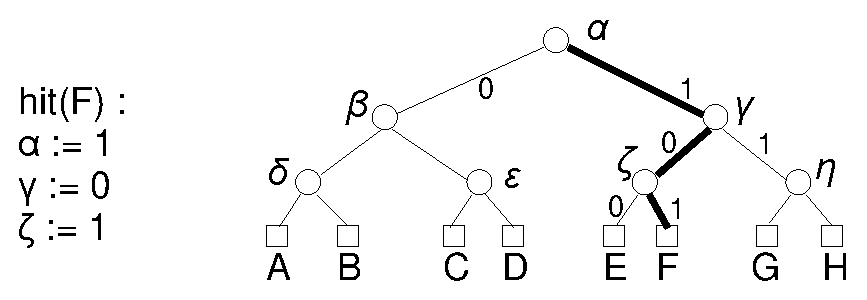
\includegraphics[width=0.7\textwidth]{2.theor/plruhit}\\
  \caption{Попадание для стратегия вытеснения \PseudoLRU
  (8-ассоциативная таблица)}\label{pseudo_lru_hit}
\end{figure}

На основании пометок вершин определяется и листовая вершина вытесняемой строки.
%Вытесняющий тег помещается в дереве на место вытесняемого.
Из корня дерева строится <<вытесняющий путь>> (он будет единственным), он приводит к вытесняемой строке. Начинает <<вытесняющий путь>> строиться из корневой вершины. Далее в <<вытесняющем пути>> исходящая дуга каждой вершины имеет пометку, противоположную пометке этой вершины. Т.е. если вершина помечена цифрой 0, значит дуга пути из этой вершины идет вправо, если вершина помечена цифрой 1 -- влево. Пример того, как определяется вытесняемая строка, показан на рис.~\ref{pseudo_lru_miss}. Цветом показаны пометки нелистовых вершин: черным
вершинам соответствует пометка 1, белым -- 0. В изображенном на рисунке дереве в качестве вытесняемой строки будет выбрана строка D, к которой ведет путь $\alpha-\beta-\varepsilon$.

\begin{figure}[h] \center
  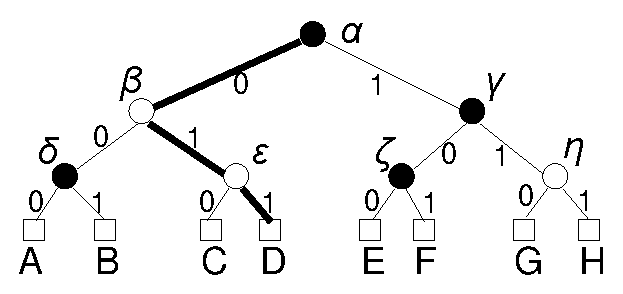
\includegraphics[width=0.5\textwidth]{2.theor/plrumiss}\\
  \caption{Определение вытесняемого элемента для стратегия вытеснения
  \PseudoLRU (8-ассоциативная таблица)}\label{pseudo_lru_miss}
\end{figure}


\subsubsection{Каноническое определение \PseudoLRU на битовой строке}

Для каждого региона хранится битовая строка $\beta$ длины $w{-}1$, где $w$ --
ассоциативность таблицы. Стратегия вытеснения определяется как процесс изменения
бит этой битовой строки.

Во многих книгах приводятся следующее определение стратегии
вытеснения \PseudoLRU для случая
$w=4$~\cite{FundamentalOfComputerOrganizationAndDesign} (в этом
случае для каждого региона выделяется 3 бита $B_1$, $B_2$ и $B_3$):
$$ \left[
  \begin{array}{c|ccc}
          & B_1 & B_2 & B_3 \\ \hline
    \pi_0 & 0 & 0 & \textsf{X} \\
    \pi_1 & 0 & 1 & \textsf{X} \\
    \pi_2 & 1 & \textsf{X} & 0 \\
    \pi_3 & 1 & \textsf{X} & 1 \\
  \end{array}
\right]
$$

Строки в регионе пронумерованы числами от 0 до $w{-}1$. При попадании на строку
региона с номером $i$ задействована строка матрицы, начинающаяся с $\pi_i$. Биты
$\beta$, напротив которых в строке матрицы находится \textsf{X}, не меняются.
Биты $\beta$, напротив которых в $i$'й строке находится число, принимают
значение, равное этому числу.

При промахе надо определить номер вытесняемой строки. Для этого используется
инвертированная форма той же матрицы (если элемент исходной матрицы был равен 0, то в инвертированной он равен 1; если в исходной равен 1, то в инвертированной равен 0; если в исходной равен \textsf{X}, то в инвертированной равен \textsf{X}):
$$
\left[
  \begin{array}{ccc|c}
    B_1 & B_2 & B_3 & \\ \hline
    1 & 1 & \textsf{X} & \rightarrow \pi_0 \\
    1 & 0 & \textsf{X} & \rightarrow \pi_1 \\
    0 & \textsf{X} & 1 & \rightarrow \pi_2 \\
    0 & \textsf{X} & 0 & \rightarrow \pi_3 \\
  \end{array}
\right]
$$

Выбирается строка матрицы, соответствующая текущему состоянию бит $B_1$,
$B_2$ и $B_3$, следующим образом: если напротив бита в строке матрицы находится число, бит
должен быть равен этому числу -- если напротив бита в строке матрицы
находится \textsf{X}, то соответствующий бит может иметь любое значение. Для любого набора значений $(B_1 B_2 B_3)$ подходящая строка матрицы всегда будет существовать и она будет единственной. Эта строка матрицы определяет вытесняемую строку региона.

Изменение $\beta$ обычно демонстрируют на бинарном дереве. Это то же дерево, что и в каноническом определении \PseudoLRU <<на бинарном дереве>>. $\beta$ составляется из пометок вершин дерева, начиная с корня и далее по слоям от левых к правым вершинам <<обходом в ширину>> (см. рис.~\ref{plru_bittree}).

\begin{figure}[h] \center
  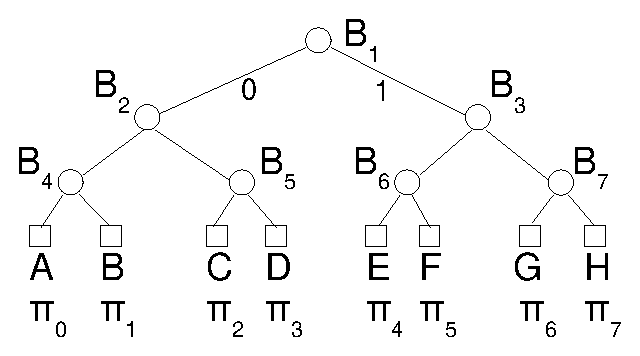
\includegraphics[width=0.5\textwidth]{2.theor/plru}\\
  \caption{Битовая строка в бинарном дереве}\label{plru_bittree}
\end{figure}

Формализованное описание для всех допустимых $w$ в литературе не
приводится. Однако в дальнейшем для формулирования и доказательства
утверждений про стратегию вытеснения \PseudoLRU такое описание будет
необходимо. Для $w=8$ изменение битовой строки будет задаваться следующей матрицей:
$$
\left[
  \begin{array}{c|ccccccc}
          & B_1 & B_2 & B_3 & B_4 & B_5 & B_6 & B_7 \\ \hline
    \pi_0 & 0 & 0 & \textsf{X} & 0 & \textsf{X} & \textsf{X} & \textsf{X} \\
    \pi_1 & 0 & 0 & \textsf{X} & 1 & \textsf{X} & \textsf{X} & \textsf{X} \\
    \pi_2 & 0 & 1 & \textsf{X} & \textsf{X} & 0 & \textsf{X} & \textsf{X} \\
    \pi_3 & 0 & 1 & \textsf{X} & \textsf{X} & 1 & \textsf{X} & \textsf{X} \\
    \pi_4 & 1 & \textsf{X} & 0 & \textsf{X} & \textsf{X} & 0 & \textsf{X} \\
    \pi_5 & 1 & \textsf{X} & 0 & \textsf{X} & \textsf{X} & 1 & \textsf{X} \\
    \pi_6 & 1 & \textsf{X} & 1 & \textsf{X} & \textsf{X} & \textsf{X} & 0 \\
    \pi_7 & 1 & \textsf{X} & 1 & \textsf{X} & \textsf{X} & \textsf{X} & 1 \\
  \end{array}
\right]
$$

Следующее утверждение~\ref{wMinus1PseudoLRU} дает алгоритм
преобразования битовой строки\\ $B_1, B_2, ..., B_{w{-}1}$ в результате
обращения в таблицу. В его формулировке будет применяться двоичное
разложение целых неотрицательных чисел от старших бит к младшим. Оно будет обозначаться для целого неотрицательного $x$ как $(x_1 x_2 ... x_n)_2$, где $x_i \in \{0, 1\}$ для $i = 1, 2, ..., n$, такие, что $x = x_n + 2{\cdot}x_{n-1} + 4{\cdot}x_{n-2} + \dots + 2^n{\cdot}x_1$. Например, 1 = (0 0 1)$_2$, 6 = (1 1 0)$_2$.

Обозначим символом $W$ выражение $\log_2 w$. По определению
стратегии вытеснения \PseudoLRU $W$ будет натуральным числом.

\begin{utv}[$(w{-}1)$-представление стратегии вытеснения
\PseudoLRU]\label{wMinus1PseudoLRU}При попадании по строке региона с номером $i = (i_1~i_2~\dots~i_W)_2$ происходит следующее изменение битовой строки $B_1,
B_2, ..., B_{w{-}1}$:

\parbox{0.3\textwidth}{
  $$ \begin{array}{l}
  B_{k_1} := i_1 \\
  B_{k_2} := i_2 \\
  B_{k_3} := i_3 \\
  ...\\
  B_{k_W} := i_W \\
  \end{array}$$
} \vline
\parbox{0.7\textwidth}{
  $$ \begin{array}{l}
  k_1 = (1)_2 \\
  k_2 = (1~i_1)_2 \\
  k_3 = (1~i_1~i_2)_2 \\
  ...\\
  k_W = (1~i_1~i_2~\dots~i_{W{-}1})_2 \\
  \end{array} $$
}
\\[1cm]

При промахе номер вытесняемой строки региона $j = (j_1~j_2~\dots~j_W)_2$ определяется следующим образом:

\parbox{0.3\textwidth}{
  $$ \begin{array}{l}
  i_1 = \neg B_{k_1} \\
  i_2 = \neg B_{k_2} \\
  i_3 = \neg B_{k_3} \\
  ...\\
  i_W = \neg B_{k_W} \\
  \end{array}$$
} \vline
\parbox{0.7\textwidth}{
  $$ \begin{array}{l}
  k_1 = (1)_2 \\
  k_2 = (1~\neg B_{k_1})_2 \\
  k_3 = (1~\neg B_{k_1}~\neg B_{k_2})_2 \\
  ...\\
  k_W = (1~\neg B_{k_1}~\neg B_{k_2}\dots\neg B_{k_{W{-}1}})_2 \\
  \end{array} $$
}
\\[0.5cm]

Кроме того при промахе делается такое же преобразование бит $B_1$, $B_2$, ..., $B_{w{-}1}$, как и в случае попадания на строку с номером $j$.
\end{utv}

Прямой проверкой нетрудно убедиться, что это утверждение верно для $w$ = 4 и 8.

\subsubsection{Определение \PseudoLRU на ветвях бинарного
дерева}\label{sec:PseudoLRUonBranches}

Здесь будет показано, как из канонических определений \PseudoLRU
получить формулировку \PseudoLRU с точки зрения одной строки региона~\cite{my_lomonosov_2010}
(в канонических определениях рассматривается весь регион целиком и
для него формулируются правила работы с последовательностью бит $B_1,
B_2, ..., B_{w{-}1}$ или пометками вершин бинарного дерева). Описываемое в этом разделе определение \PseudoLRU ранее не встречалось в литературе.

Сначала этот переход покажем в частном случае, на примере $w=4$. Первый шаг --- это
смена <<состояния>>: вместо последовательности бит $B_1, B_2, ...,
B_{w-1}$ будем рассматривать последовательность векторов бит
$\beta_0, \beta_1, \dots, \beta_{w-1}$, каждый $\beta_i$ --- это вектор из $W$ бит. Каждый $\beta_i$ соответствует $i$'й листовой вершине бинарного дерева (см. рисунок~\ref{fig:plru_def_step1}). Попадание
меняет теперь атрибуты не внутренних вершин дерева $(B_1 B_2 B_3)$, а листовых $(\beta_0 ... \beta_3)$.
Каждый $\beta_i$ будет представляться списком длины $W$, обозначающим путь от
корня дерева к $i$'й листовой вершине: $\beta_0$ соответствует
($B_1$ $B_2$), $\beta_1$ соответствует ($B_1$ $\neg B_2$), $\beta_2$
соответствует ($\neg B_1$ $B_3$) и $\beta_3$ соответствует ($\neg
B_1$ $ \neg B_3$).\\[0.5cm]

\begin{figure}[h]
\parbox{0.2\textwidth}{ \centering
  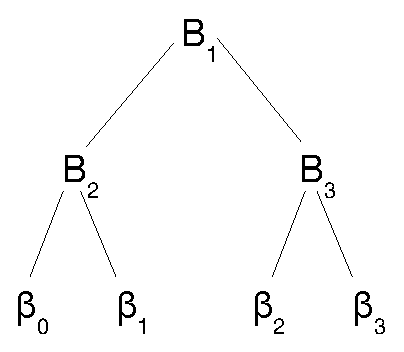
\includegraphics[width=0.2\textwidth]{1.review/btree}
}
\parbox{0.25\textwidth}{
$$ \left[
  \begin{array}{c|ccc}
          & B_1 & B_2 & B_3 \\ \hline
    \pi_0 & 0 & 0 & \textsf{X} \\
    \pi_1 & 0 & 1 & \textsf{X} \\
    \pi_2 & 1 & \textsf{X} & 0 \\
    \pi_3 & 1 & \textsf{X} & 1 \\
  \end{array}
\right]
$$
} $\stackrel{1}{\longrightarrow}$ %\vline
\parbox{0.4\textwidth}{
$$ \left[
  \begin{array}{c|cccc}
          & \beta_0 & \beta_1 & \beta_2 & \beta_3 \\ \hline
    \pi_0 & (0~0) & (0~1) & (1~\textsf{X}) & (1~\textsf{X}) \\
    \pi_1 & (0~1) & (0~0) & (1~\textsf{X}) & (1~\textsf{X}) \\
    \pi_2 & (1~\textsf{X}) & (1~\textsf{X}) & (0~0) & (0~1) \\
    \pi_3 & (1~\textsf{X}) & (1~\textsf{X}) & (0~1) & (0~0) \\
  \end{array}
\right]
$$
}
\caption{Смена состояния}\label{fig:plru_def_step1}
\end{figure}

Заметим, что получилась симметричная матрица. На пересечении $\pi_i$
и $\beta_j$ располагается вектор, задающий изменение $\beta_j$ (вектора в $j$'й
листовой вершине дерева) при попадании по строке региона, соответствующей $i$'й листовой вершине дерева. Назовем позицию $i \oplus j$ \emph{относительной позицией}
$i$ относительно $j$. Рассмотрим отдельно каждый столбец
получившейся матрицы (на рисунке~\ref{fig:plru_def_step2} до стрелки) и упорядочим строки столбцов в порядке увеличения относительных позиций (на рисунке~\ref{fig:plru_def_step2} после стрелки).

\begin{figure}[h]
\parbox{0.2\textwidth}{
$$ \left[
  \begin{array}{c|c}
          & \beta_0 \\ \hline
    \pi_0 & (0~0) \\
    \pi_1 & (0~1) \\
    \pi_2 & (1~\textsf{X}) \\
    \pi_3 & (1~\textsf{X}) \\
  \end{array}
\right]
$$
}\parbox{0.2\textwidth}{
$$ \left[
  \begin{array}{c|c}
          & \beta_1 \\ \hline
    \pi_0 & (0~1) \\
    \pi_1 & (0~0) \\
    \pi_2 & (1~\textsf{X}) \\
    \pi_3 & (1~\textsf{X}) \\
  \end{array}
\right]
$$
}\parbox{0.2\textwidth}{
$$ \left[
  \begin{array}{c|c}
          & \beta_2 \\ \hline
    \pi_0 & (1~\textsf{X}) \\
    \pi_1 & (1~\textsf{X}) \\
    \pi_2 & (0~0) \\
    \pi_3 & (0~1) \\
  \end{array}
\right]
$$
}\parbox{0.2\textwidth}{
$$ \left[
  \begin{array}{c|c}
          & \beta_3 \\ \hline
    \pi_0 & (1~\textsf{X}) \\
    \pi_1 & (1~\textsf{X}) \\
    \pi_2 & (0~1) \\
    \pi_3 & (0~0) \\
  \end{array}
\right]
$$
} $\stackrel{2}{\stackrel{\longrightarrow}{\pi^i_j \equiv \pi_{i
\oplus j}}}$

\parbox{0.24\textwidth}{
$$ \left[
  \begin{array}{c|c}
          & \beta_0 \\ \hline
    \pi^0_0 \equiv \pi_0 & (0~0) \\
    \pi^0_1 \equiv \pi_1 & (0~1) \\
    \pi^0_2 \equiv \pi_2 & (1~\textsf{X}) \\
    \pi^0_3 \equiv \pi_3 & (1~\textsf{X}) \\
  \end{array}
\right]
$$
}\parbox{0.24\textwidth}{
$$ \left[
  \begin{array}{c|c}
          & \beta_1 \\ \hline
    \pi^1_0 \equiv \pi_1 & (0~0) \\
    \pi^1_1 \equiv \pi_0 & (0~1) \\
    \pi^1_2 \equiv \pi_3 & (1~\textsf{X}) \\
    \pi^1_3 \equiv \pi_2 & (1~\textsf{X}) \\
  \end{array}
\right]
$$
}\parbox{0.24\textwidth}{
$$ \left[
  \begin{array}{c|c}
          & \beta_2 \\ \hline
    \pi^2_0 \equiv \pi_2 & (0~0) \\
    \pi^2_1 \equiv \pi_3 & (0~1) \\
    \pi^2_2 \equiv \pi_0 & (1~\textsf{X}) \\
    \pi^2_3 \equiv \pi_1 & (1~\textsf{X}) \\
  \end{array}
\right]
$$
}\parbox{0.24\textwidth}{
$$ \left[
  \begin{array}{c|c}
          & \beta_3 \\ \hline
    \pi^3_0 \equiv \pi_3 & (0~0) \\
    \pi^3_1 \equiv \pi_2 & (0~1) \\
    \pi^3_2 \equiv \pi_1 & (1~\textsf{X}) \\
    \pi^3_3 \equiv \pi_0 & (1~\textsf{X}) \\
  \end{array}
\right]
$$
}
\caption{Нумерация относительными позициями}\label{fig:plru_def_step2}
\end{figure}

После перехода к относительным позициям ($\pi^i_j$ -- это позиция
$\pi_j$ относительно $\pi_i$, т.е. $\pi_{i \oplus j}$) все столбцы получились одинаковыми.
Иными словами, \emph{алгоритм изменения порядка строк региона согласно стратегии
вытеснения \PseudoLRU на относительных позициях инвариантен
относительно абсолютной позиции вытесняемой строки}. Следующая теорема
формально доказывает этот факт.

Будем называть \emph{\PseudoLRU-ветвью позиции $i$} вектор
$(B_{k_1}^{\sigma_1}~B_{k_2}^{\sigma_2}~\dots~B_{k_W}^{\sigma_W})$,
в котором $k_1 = (1)_2, \sigma_1 = \neg i_1, \sigma_j = \neg i_j$, $k_j = (1~i_1~i_2~\dots~i_{j-1})_2$, $j = 2, 3, \dots, W$, $i = (i_1~i_2~\dots~i_W)_2$. Степени определены стандартным образом: $B^1 \equiv B, B^0 \equiv \neg B$. Например, \PseudoLRU-ветвью позиции 0 есть $(B_1 B_2 B_4 ...)$. Каждой строке региона (т.е. каждой позиции строк региона) соответствует своя \PseudoLRU-ветвь. Каждое обращение изменяет все ветви некоторым образом, который не зависит от абсолютной позиции, а зависит от относительной:

\begin{theorem}[Инвариантность преобразования \PseudoLRU-ветвей относительными
позициями]\label{thm_pseudoLRU_invariant} \PseudoLRUInvariant
\end{theorem}
Доказательство теоремы приведено в приложении~\ref{sec:proofs}.

Доказанный факт позволяет сформулировать определение стратегии
вытеснения \PseudoLRU, сфокусированное не на изменении атрибутов строк всего
региона,
а на изменении атрибутов одной строки. На этом определении
будут базироваться применения предлагаемых методов генерации
ограничений для стратегии вытеснения \PseudoLRU.

\begin{utv}[формулировка \PseudoLRU на ветвях бинарного дерева]
Сопоставим некоторой произвольной строке региона вектор длины $W$. Каждое обращение к этой строке региона делает её вектор равным (0 0 ... 0). Строка региона является вытесняемой, если её вектор равен (1 1 ... 1).
Влияние других обращений определяется относительной позицией их
строки региона относительно позиции данной строки региона. Если относительная позиция
принадлежит области $[\frac{w}{2^k},~\frac{w}{2^{k-1}}), k =
1,2,...,W$, то первые $k{-}1$ элементов битового вектора становятся равными
0, $k$'й элемент вектора становится равным 1, остальные элементы
вектора не меняются. Если относительная позиция равна 0, то все элементы вектора становятся равными 0.
\end{utv}

Битовый вектор длины $W$ будет соответствовать пути из корня бинарного
дерева в листовую вершину, соответствующую данной строке региона.
Удобно представлять процесс изменения элементов бинарного вектора  в виде их
\emph{перекрашивания}. Про элементы битового вектора, равные 0,
будем говорить, что они покрашены в \emph{белый} цвет, а элементы вектора, равные 1, --- в\emph{черный}.

Говоря в терминах бинарного дерева из канонических определений \PseudoLRU, каждое обращение в регион изменяет пометки в нелистовых вершинах дерева. Каждой листовой вершине соответствует единственный в нее путь из корня дерева (та самая <<ветвь>>). Вершина дерева, входящая в ветвь, с точки зрения этой ветви будет <<белой>>, если пометка этой вершины совпадает с направлением дуги дерева из этой вершины. входящей в ветвь, <<черной>> --- если не совпадает. Вытесняется та строка региона, путь к которой полностью состоит из несоответствующих дуг по каноническим определениям, т.е. из черных вершин по новому определению. На рисунке~\ref{recolor}
изображен процесс перекрашивания ветви, ведущей в А, под действием
попадания в C (для сокращения показана только ветвь в А без
остальной части дерева). Так как путь из корня в C совпадает из
верхних двух вершин, то они перекрашиваются в белый цвет. Дуга из
третьей вершины пути в С не совпадает с дугой пути в А, поэтому
третья вершина перекрашивается в черный цвет. Остальные вершины
ветви остаются без изменений.

\begin{figure}[h] \center
  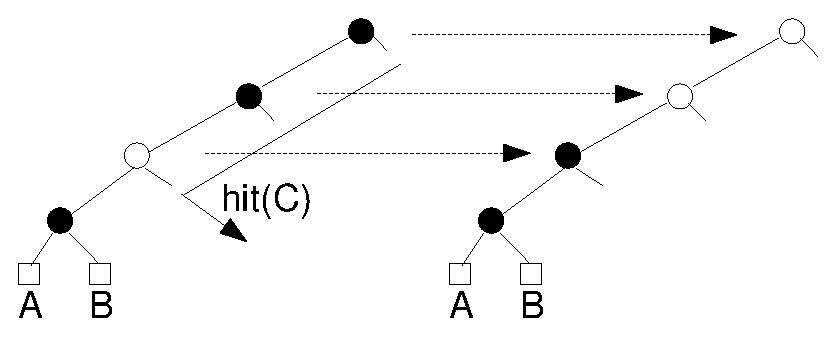
\includegraphics[width=0.8\textwidth]{1.review/recolor}\\
  \caption{Перекрашивание ветви в А}\label{recolor}
\end{figure}


Определение стратегии вытеснения \PseudoLRU на ветвях дерева
является связующим звеном между каноническим определением (например,
на битовой строке) и определением с помощью таблицы вытеснения,
поскольку ветвь -- это и есть двоичное разложение позиции, которая меняется точно так же, как и позиция в перестановке согласно таблице вытеснения.


%%%%%%%%%%%%%%%%%%%%%%%%%%%%%%%%%%%%%%%%%%%%%%%%%%%%%%%%%%%%%%%%%%%%

\section{Метод полезных обращений для записи стратегии вытеснения в виде ограничений}\label{sec:usefulness_functions}

%{\footnotesize В разделе рассматривается метод составления ограничений для
%описания стратегии вытеснения, для которой удается определить функционал
%вытеснения. Стратегия вытеснения описывается ограничением сверху на количество \emph{полезных} инструкций (т.е. помогающих вытеснению).
%В разделе приведены определения полезных инструкций и способы составления ограничений для трех
%наиболее часто используемых в микропроцессорах стратегий вытеснения -- \LRU, \FIFO и \PseudoLRU. Освещается понятие \emph{монотонного функционала вытеснения}, который является залогом более
%простой системы ограничений.}

В данном разделе процесс вытеснения будет представляться как изменение  системы функций, отображающих ключи в целые числа. Каждое обращение в таблицу изменяет значения функций по всем ключам\footnote{это напоминает изменение операций в рамках машин абстрактного состояния Ю.Гуревича~\cite{ASM}}. Пример процесса изменения значения функции для некоторого ключа изображен на рисунке~\ref{fig:graphic}.

\begin{figure}[h] \center
  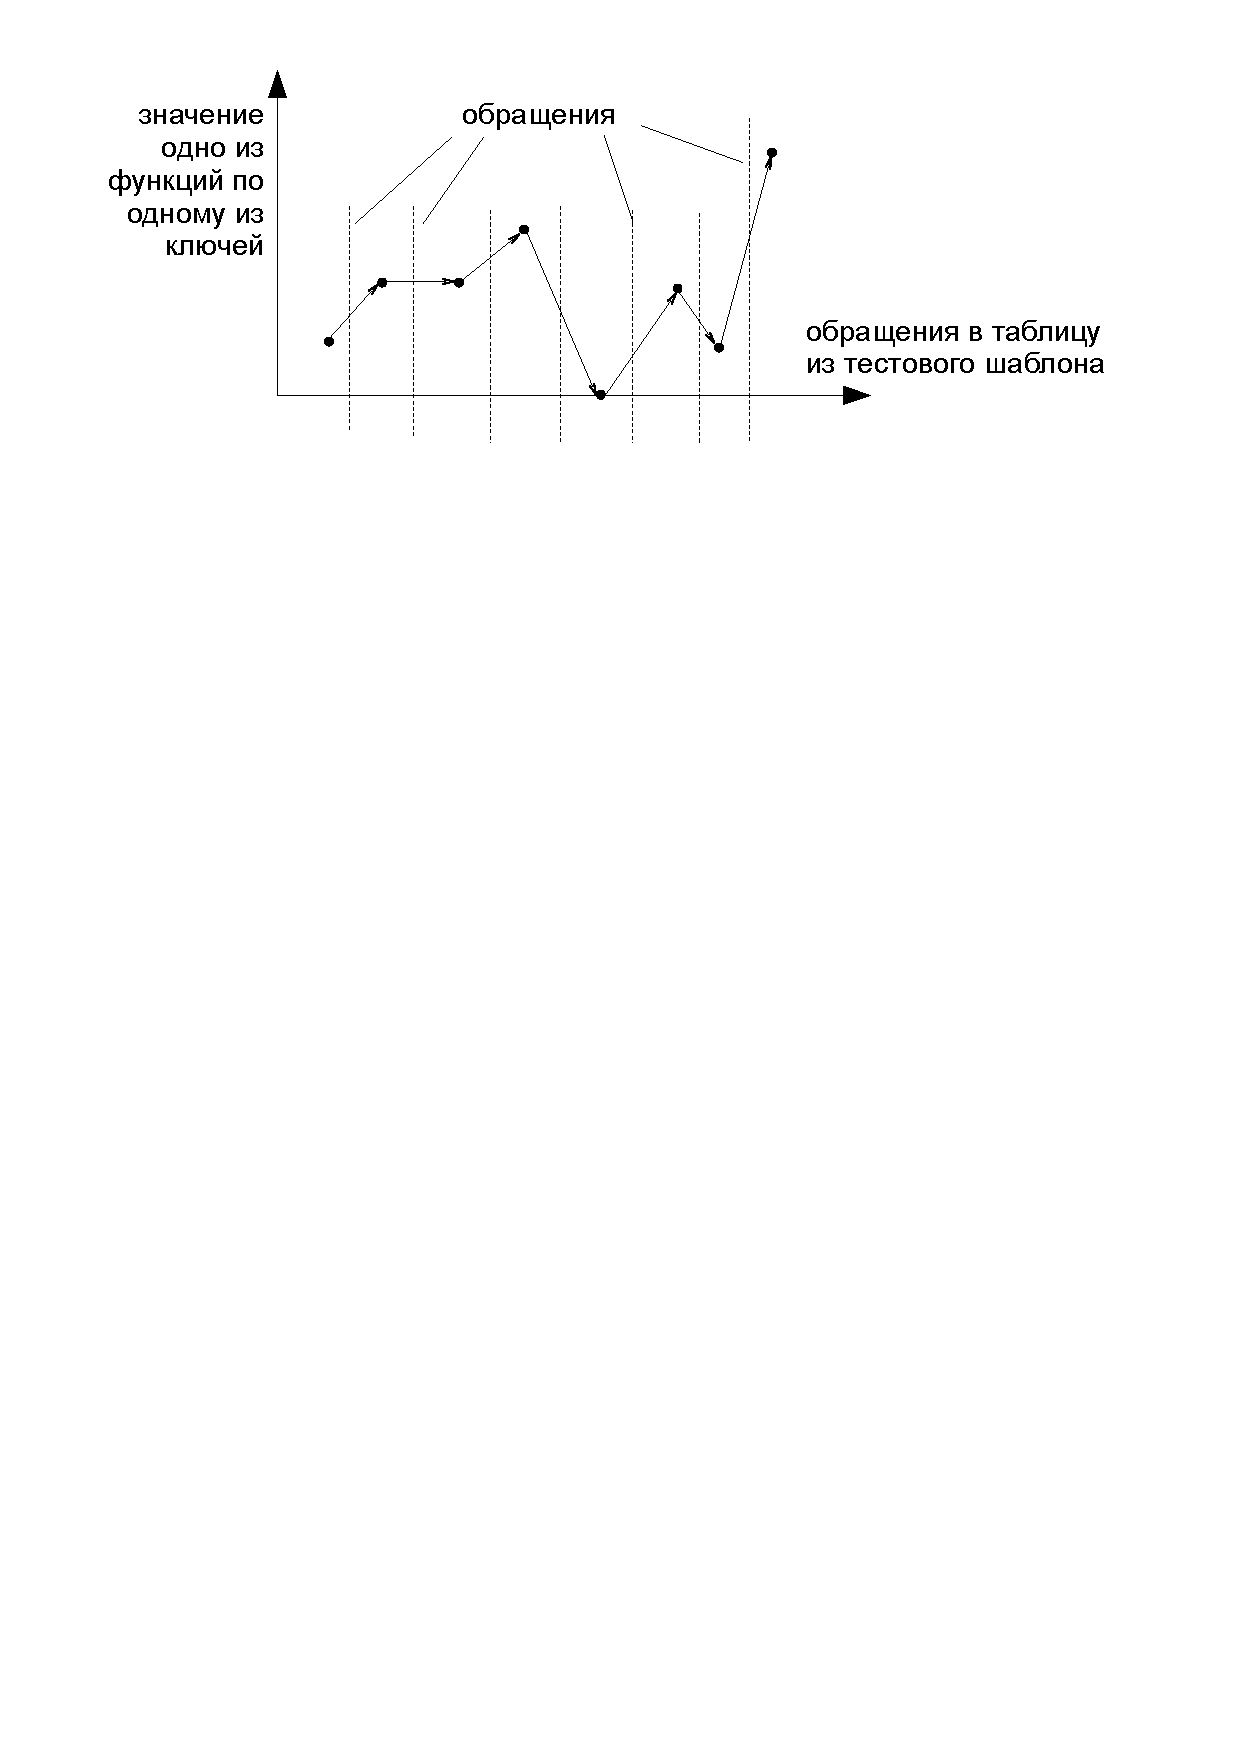
\includegraphics[width=0.7\textwidth]{2.theor/graphic}\\
  \caption{К определению стратегии вытеснения}\label{fig:graphic}
\end{figure}

Говоря формально, пусть $\alpha, \beta, \dots, \gamma$ --- одноместные функции,
отображающие ключи в целые числа. Для каждого обращения определены функции
изменения значений функций $\alpha, \beta, \dots, \gamma$ (если не сказано иное, будет предполагаться, что обращения осуществляются в один и тот же регион):
$$\parbox{2.5cm}{in-parallel\\forall keys x~}\left|\begin{array}{l}
\alpha(x) := A_I(k, \alpha, \beta, \dots, \gamma)\\
\beta(x) := B_I(k, \alpha, \beta, \dots, \gamma)\\
\dots\\
\gamma(x) := C_I(k, \alpha, \beta, \dots, \gamma)\\
\end{array}\right.
$$

Обновления значений функций $\alpha, \beta, \dots, \gamma$ выполняются одновременно. $I$ --- обращение в таблицу, $k$ --- ключ в этом обращении. Функции $A_I$, $B_I$, \dots, $C_I$ отражают влияние обращения по некоторому ключу на другой произвольный ключ. $x$ --- это ключ, за которым <<следим>> и условия вытеснения которого нас интересуют, а $k$ ---это ключ в очередном обращении из тестового шаблона.
Возможны следующие случаи (в качестве $x$ рассматривается произвольный ключ, не
обязательно <<находящийся>> в регионе):
\begin{itemize}
    \item в результате обращения по ключу $k$ ключ $x$ <<попадает>> в регион (т.е. в регион добавляется строка с ключом $x$);
    \item в результате обращения по ключу $k$ ключ $x$ <<вытесняется>> из региона (т.е. из региона удаляется строка с ключом $x$);
    \item в результате обращения по ключу $k$ <<состояние>> ключа $x$ в регионе не меняется.
\end{itemize}

%Этим ситуациям как раз и ставятся в соответствие классы значений функций $\alpha, \beta, \dots, \gamma$, а функции $A_I$, $B_I$, \dots, $C_I$ осуществляют переход между этими классами. Тем самым стратегия вытеснения будет описана в виде изменения таких <<счетчиков>> $\alpha, \beta, \dots, \gamma$.

%Формально это правило выражается следующим образом.
Будем называть функцию
$\alpha$, отображающую ключи в целые числа, \emph{функционалом вытеснения} для заданной стратегии вытеснения, если одновременно выполнены следующие свойства:
\begin{enumerate}
  \item существуют константы $\alpha_{min}$ и $\alpha_{max}$ такие, что
$\alpha_{min} \leqslant \alpha_{max}$;
  \item для любого ключа $x$ $\alpha_{min} \leqslant \alpha(x) \leqslant
\alpha_{max}$ тогда и только тогда, когда $x$ находится в регионе по определению
стратегии вытеснения (т.е. <<был помещен>> в регион и до сих пор не вытеснен);
  \item для любого ключа $k$ $A_I(k, \alpha,\beta,\dots,\gamma) (k) =
\alpha_{min}$;
  \item $\exists! \varphi: \mbox{~ключ~} \times \mathds{Z}^{n} \times \mbox{~ключ~} \times \mathds{Z}^{n} \rightarrow
\mathds{Z}$, где $n$ --- количество функций во множестве
$\{\alpha,\beta,\dots,\gamma\}$, такая, что для любого ключа $x$ $$A_I(k,
\alpha,\beta,\dots,\gamma)(x) \equiv \varphi(k, \alpha(k), \beta(k), \dots,
\gamma(k), x, \alpha(x), \beta(x), \dots, \gamma(x))$$ иными словами, в функции
изменения функционала вытеснения разрешается обращаться только к $k$ и тому ключу,
для которого определяется функционал вытеснения;
  \item $\exists!$ ключ $x^* : \alpha(x^*) = \alpha_{max}$;
  \item перед любым неуспешным обращением $\alpha(x^*) =
\alpha_{max}$ тогда и только тогда, когда $x^*$ есть <<вытесняемый>> ключ по
определению стратегии вытеснения (т.е. строка с ключом $x^*$ является
вытесняемой при данном обращении по определению стратегии вытеснения);
\end{enumerate}

Пример функционала вытеснения: $\alpha$ --- счетчик количества обращений к строке
для стратегии вытеснения \LRU. Обращение по тому же ключу делает $\alpha$
равным 1, по другому ключу --- увеличивает $\alpha$ на единицу. Вытесняемым
считается ключ, чей счетчик равен $w$ --- количеству строк в регионе. Проверим
определение функционала вытеснения:
\begin{enumerate}
    \item $\alpha_{min}$ = 1, $\alpha_{max}$ = $w$, $1 \leqslant w$;
    \item верно, что счетчик больше $w$ тогда и только тогда, когда $x$ не
находится в регионе; в противном случае, было бы возможно подряд успешно обратиться к
большему числу строк, чем хранится в регионе;
    \item по условию обращение по тому же ключу делает $\alpha$ равным 1, что
и есть $A_I(x;...)(x) = 1$;
    \item изменение одного счетчика производится независимо от изменений других счетчиков (хотя, конечно, все счетчики изменяются одновременно);
    \item такой $x^*$ существует, ибо в противном случае было бы возможно подряд успешно обратиться к большему числу строк, чем хранится в регионе; такой $x^*$ единственный, поскольку каждое обращение меняет каждый счетчик и в минимальное значение $\alpha$ изменяется лишь по единственному ключу.
\end{enumerate}

Пусть для стратегии вытеснения сформулирован функционал вытеснения. Будем называть
обращение по некоторому ключу \emph{полезным для вытеснения} ключа
$x$ (или просто, \emph{полезным}), если оно монотонно увеличивает функционал вытеснения по
ключу $x$ до максимального значения (см. рис.~\ref{useful}).\\

\begin{figure}[h] \center
  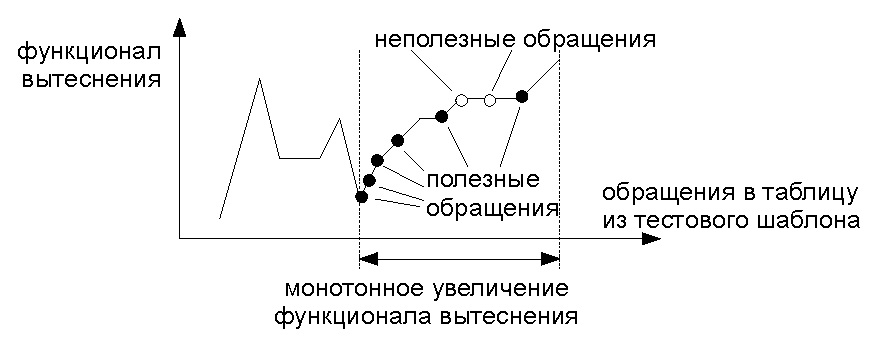
\includegraphics[width=0.6\textwidth]{2.theor/useful}\\
  \caption{К определению полезных обращений}\label{useful}
\end{figure}

Тогда вытеснение будет происходить в том случае, когда количество
полезных обращений превысит некоторое константное количество.
И вытеснение не будет происходить, если это количество не превысит некоторой константной верхней границы.

\emph{Формулой полезного обращения} будем называть предикат от вытесняемого ключа $k$ и региона $R$ и ключей и регионов предыдущих обращений, при которых это обращение будет полезным для вытеснения ключа $k$ из региона $R$.

Тем самым ограничение (constraint) <<быть вытесненным>> представимо в виде
ограничения сверху на <<сумму>> формул полезных обращений по всем предыдущим обращениям: $\sum_{i=1}^n [u_x(k_i)] < N$, где $u_x(k_i)$ -- формула полезного обращения по ключу $k_i$ для ключа $x$ в полностью ассоциативной таблице, для остальных таблиц будут указываться регионы обращений: $u_{x,r}(k_i, r_i)$.

Формулы полезных обращений, как и функционалы вытеснения, не являются единственными. Например, для стратегии вытеснения \LRU возможны следующие две различные формулы полезных обращений (далее для одной из них будет формально показано, что она действительно задает полезные обращения) (формулы приведены для случая полностью ассоциативной таблицы):
\begin{itemize}
  \item $u_x(x_i) \equiv (x \notin \{x_i, x_{i+1}, ..., x_n\} \wedge
\bigwedge\limits_{j=1}^{i-1} (x \in \{x_j, x_{j+1}, ..., x_{i-1}\} \vee x_j
\neq x_i))$ -- обращение считается полезным, если оно расположена после
последнего обращения к $x$ и с того момента является первым обращением к своему
ключу; нетрудно заметить, что это в чистом виде определение \LRU, изображенное на рисунке~\ref{fig:lru1}: обращение по ключу $x_j$, который расположен после ключа $x$, передвигает $x$ к концу вектора, за концом происходит вытеснение; первые обращения по ключам после последнего обращения к $x$ -- это и есть именно те обращения, где $x$ сдвигается к концу; иначе говоря, полезное обращение сдвигает $x$ к концу, приближая его к вытеснению;
  \item $u_x(x_i) \equiv (x \notin \{x_i, x_{i+1}, ..., x_n\} \wedge x_i \notin
\{x_{i+1}, x_{i+2}, ..., x_n\})$ -- обращение считается полезным, если оно
расположено после последнего обращения к $x$ и является последним обращением к
своему ключу перед финальным обращением к $x$; т.е. в таблице хранятся некоторые ключи, есть некоторый ключ $x$, есть последовательность других обращений (их
ключи обозначены как  $x_i$, ..., $x_n$), полезными будут лишь последние к ним обращения (среди $x_i$, ..., $x_n$ могут быть равные), т.е. все полезные обращения вместе образуют (по разу) все различные ключи.
\end{itemize}

Тем самым, метод полезных обращений состоит в следующем:
\begin{enumerate}
  \item выделить функционал вытеснения $\alpha$;
  \item выделить определение полезной инструкции;
  \item записать формулу полезного обращения $u_{x,r}(x_i, r_i)$ для обращения с ключом $x$ и регионом $r$;
  \item определить $\alpha_{max}$;
  \item составить ограничение для свойства <<$x$ вытеснен>> в виде
$\sum\limits_{i=1}^n u_{x,r}(x_i, r_i) > \alpha_{max}$ и для свойства <<$x$ не
вытеснен>> в виде $\sum\limits_{i=1}^n u_{x,r}(x_i,r_i) \leqslant \alpha_{max}$.
\end{enumerate}

Ключевой вопрос при применении метода полезных обращений --- это выбор
функционала вытеснения. От него в том числе будет зависеть сложность функции
полезности и генерируемых ограничений.

 Функционал вытеснения может быть получен из таблицы вытеснения
(policy table). А именно, если вытеснение происходит с позиции с максимальным
номером (т.е. в последней строке отсутствует число $w{-}1$), а в результате
попадания ключ переносится в самое начало (т.е. второй столбец имеет вид (0 1 2
... $w{-}1$ $m$)$^T$ ). Тогда $\alpha$ --- это позиция ключа в перестановке,
$\alpha_{min}$ = 0, $\alpha_{max} = w{-}1$. Этими свойствами, например, обладают
таблицы вытеснения \LRU (см.рис.~\ref{fig:PolicyTableLRU8}) и
\PseudoLRU~\cite{policy_tables}.

%В отличие от метода диапазонов вытеснения при использовании функций полезности не происходит выделение участка тестового шаблона, непосредственно влияющего на вытеснение. Считается, что это влияние начинается с момента появления строки в таблице. Другое дело, что одни инструкции влияют на ее вытеснение (это и есть <<полезные>> инструкции), а другие -- нет.


\subsection{Метод полезных обращений для стратегии вытеснения \LRU}

\LRU (Least Recently Used) --- это стратегия вытеснения,
определяющая вытесняемые данные как наименее используемые. Она
эффективна для алгоритмов, обладающих свойством локальности данных,
т.е. чаще использующих те данные, к которым недавно происходило
обращение. Эта стратегия используется, например, в микропроцессорах
архитектуры MIPS~\cite{mips64II}.

Стратегия вытеснения \LRU обычно определяется с использованием
счетчиков обращений. Для каждой строки таблицы
вводится счетчик обращений к ней. Каждое обращение увеличивает
счетчик. Счетчик вытесняющей строки на единицу больше максимального счетчика невытесняемых строк. Вытесняемой в регионе будет строка с минимальным счетчиком его строк.
%Поскольку границы значений счетчика неизвестны, формулирование
%функционала вытеснения на основе счетчика провести сложно.

Другой способ описания \LRU основан на введении порядка на строках региона (т.е.
регион представляется вектором строк). После каждой инструкции элементы этого вектора переупорядочиваются, \emph{переставляются}, согласно следующим правилам (см.рис.~\ref{fig:lru1}):
\begin{itemize}
\item при попадании соответствующая строка перемещается в начало, строки, которые расположены левее этой, сдвигаются на одну позицию вправо;
\item при промахе вытесняется последняя строка, в начало вставляется вытесняющая.
\end{itemize}

\begin{figure}[h] \center
  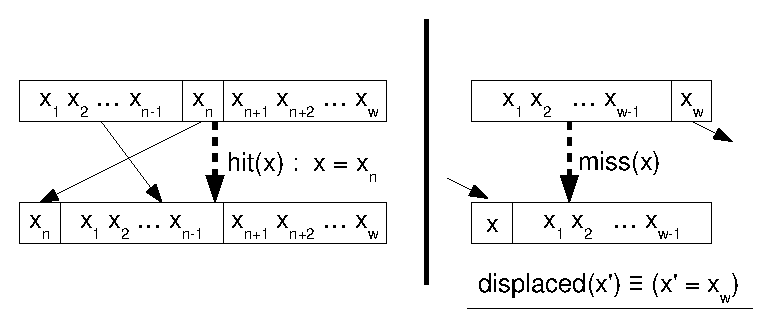
\includegraphics[width=0.6\textwidth]{2.theor/lru1}\\
  \caption{Стратегия вытеснения \LRU (w --- ассоциативность) на
перестановках}\label{fig:lru1}
\end{figure}

Позиция строки, ее индекс, в таком векторе ограничена, единственна, ее изменение допускает представление, независимое от других ключей. Тем самым \emph{<<позиция>> ключа является функционалом вытеснения}.

Функция изменения этого функционала выглядит следующим образом:\\

\parbox{0.5\textwidth}{ \tt
$A_{\mbox{hit}}(k, \alpha)(x) \equiv$\\
if $\alpha(x) > w$ then $\alpha(x)$\\
elsif $\alpha(k) > \alpha(x)$ then $\alpha(x)+1$\\
elsif $\alpha(k) = \alpha(x)$ then $1$\\
else $\alpha(x)$ endif%
}\parbox{0.5\textwidth}{\tt
$A_{\mbox{miss}}(k, \alpha)(x) \equiv$\\
if $k = x$ then $1$\\
elsif $\alpha(x) > w$ then $\alpha(x)$\\
else $\alpha(x) + 1$ endif}\\

Полезным будет считаться обращение, увеличивающее позицию, т.е.
переставляющее соответствующий ключ к концу. Такими обращениями являются все
промахи (поскольку они вытесняют последнюю строку вектора с передвижением всех остальных на одну позицию к концу, т.е. будет передвинута и строка с ключом $x$) и
попадания к строкам, находившимся ближе к концу, чем $x$ (потому как при попадании они передвинутся в самое начало, а все строки от начала и до них сдвинутся на одну
позицию к концу, в том числе и $x$).

Осталось выразить эту идею в виде ограничений~\cite{my_ewdts_2009}.
Учет полезных обращений начинается уже в инициализирующей последовательности,
тем самым необходимо будет сформулировать формулы полезных обращений и для
инициализирующих обращений.

Следующая теорема описывает функцию полезности для \LRU ($m$ --- количество
инициализирующих инструкций):

\begin{theorem}[Выражение свойства <<быть вытесненным>> для \LRU]\label{correct_mirror_LRU} \LRUusefuls
\end{theorem}

\begin{proof}
По определению стратегии вытеснения \LRU <<$k$ не вытеснен из региона $R$ согласно определению на перестановках>> эквивалентно тому, что после последнего обращения к $k$ в $R$ происходит не более $w$ обращений по различным ключам в регион $R$. Несложно убедиться, что это количество выражается следующей формулой: $$|\{s_i| R = R(s_i) \wedge s \notin \{s_i, ..., s_{m+n}\}\}|$$
Однако это же число можно записать другим образом, чтобы исключить повторения одинаковых $s_i$:
$$|\{s_i| R = R(s_i) \wedge s \notin \{s_i, ..., s_{m+n}\} \wedge s_i \notin \{s_{i+1}, ..., s_{m+n}\}\}|$$

Ввиду конечности последовательности $\langle s_i, ..., s_{m+n}\rangle$ в нем всегда найдется последнее вхождение $s_i$ --- множество последних вхождений всех элементов списка равно множеству всех элементов списка.

Представленная мощность множества и есть требуемая сумма.
\end{proof}

Из теоремы~\ref{correct_mirror_LRU} следует система ограничений для
описания обращений по ключу $k_i$ в регион $R_i$ согласно методу полезных обращений для \LRU: \begin{itemize}
\item для hit($k_i, R_i$):
$$
\left\{\begin{array}{l} (k_i||R_i) \in \{(t_1||r_1), ..., (t_m||r_m), (k_1||R_1),
..., (k_{i-1}||R_{i-1})\}\\
\sum\limits_{j=1}^m [u_{k_i,R_i}(t_j||r_j)] + \sum\limits_{j=1}^{i-1} [u_{k_i,R_i}(k_j||R_j)] < w\\
\{(t_1||r_1), ..., (t_m||r_m)\} - \mbox{все разные}\\
\end{array} \right.
$$
\item для miss($k_i, R_i$):
$$
\left\{\begin{array}{l} (k_i||R_i) \in \{(t_1||r_1), ..., (t_m||r_m), (k_1||R_1),
..., (k_{i-1}||R_{i-1})\}\\
\sum\limits_{i=1}^m [u_{k_i,R_i}(t_j||r_j)] + \sum\limits_{j=1}^{i-1} [u_{k_i,R_i}(k_j||R_j)]
\geqslant w\\
\{(t_1||r_1), ..., (t_m||r_m)\} - \mbox{все разные}\\
\end{array} \right.
$$
\end{itemize}


%Для этого удобно использовать утверждение~\ref{hit_miss_human}. Символом
%$\lambda_\delta$ будет обозначаться элемент начального
%состояния таблицы с индексом $\delta$ по порядку \LRU, $1 \leqslant \delta \leqslant w$. Индекс 1 обозначает самый молодой элемент, индекс $w$ обозначает самый старый элемент.
%
%Применение полезностей эффективно в том случае, когда домен имеет
%небольшой размер. В этом случае можно перебрать все элементы
%домена (это и будут $\lambda_\delta$) и составить для них свои
%полезности, причем для каждого элемента будет известен индекс по
%порядку \LRU ($\delta$). Ограничение, описывающее стратегию
%вытеснения, будет при этом иметь вид дизъюнкции по элементам домена.
%
%Если вытесняемый элемент был в начальном состоянии (пусть это
%$\lambda_\delta$) и к нему не было обращений, то для его вытеснения
%необходимо $w-\delta + 1$ полезных инструкций, потому что столько
%раз надо подвинуть элемент с индексом $\delta$ в \LRU-списке в
%сторону к концу (к элементам с индексом $w$), чтобы он вышел за
%границу списка (иными словами, чтобы он был вытеснен).
%
%Если вытесняемый элемент был в начальном состоянии и к нему было
%обращение, то для его вытеснения необходимо $w$ инструкций, так как
%во время обращения элемент был поставлен в самое начало \LRU-списка.
%То же справедливо для внесенных в кэширующий буфер новых тегсетов --
%чтобы их вытеснить, надо так же $w$ полезных инструкций, чтобы
%переместить их к концу \LRU-списка.
%
%В таблице~\ref{hit_miss_table} приведены все функции полезности для
%кэш-попаданий и кэш-промахов. Доказательство корректности приведенных
% в ней формул (т.е. доказательство того, что эти формулы действительно
% описывают \LRU) важны, но не представляют самостоятельного результата.
%Поэтому они были вынесены за пределы основной части диссертации и
%находятся в приложении~\ref{sec:proofs}.

В некоторых случаях количество ограничений удается сократить, используя следующую эвристику для ограничения вида $\sum_{i=1}^n a_i \leqslant C$:
\begin{itemize}
    \item если $C > n$, то его не включать в конъюнкцию;
    \item если $C < 0$, то вся конъюнкция с этим ограничением несовместна;
    \item если $C = 0$, то его сразу расписать в конъюнкцию ограничений
$a_i = 0$ для каждого $i$ от 1 до $n$;
    \item если $C = n$, то его сразу расписать в конъюнкцию ограничений
$a_i = 1$ для каждого $i$ от 1 до $n$.
\end{itemize}

Аналогично с ограничениями вида $\sum_{i=1}^n a_i \geqslant C$.


\subsection{Метод полезных обращений для стратегии вытеснения \FIFO}

\FIFO (First-In First-Out) -- это стратегия вытеснения, определяющая
вытесняемые данные согласно принципу очереди FIFO. Например, в
микропроцессоре PowerPC 970FX вытеснение из небольшого буфера,
хранящего последние преобразованные эффективные адреса в физические,
D-ERAT, происходит согласно \FIFO~\cite{PowerPC970FXUserManual}.

Стратегия \FIFO допускает описание на основе порядка на строках
региона (т.е. регион представляется вектором строк-элементов). После каждого
обращения строки вектора переупорядочиваются, \emph{перставляются}, согласно следующим правилам
(см.рис.~\ref{fifo1}):
\begin{itemize}
\item при попадании порядок строк не меняется;
\item при промахе вытесняется последняя строка, в начало вставляется вытесняющая строка.
\end{itemize}

\begin{figure}[h] \center
  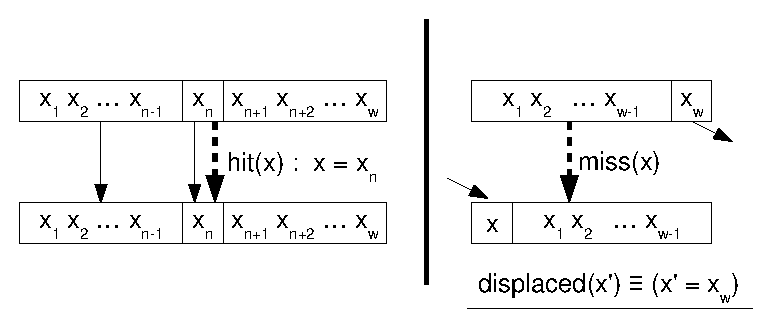
\includegraphics[width=0.6\textwidth]{2.theor/fifo1}\\
  \caption{Стратегия вытеснения \FIFO (w --- ассоциативность
таблицы)}\label{fifo1}
\end{figure}

Отличие от \LRU лишь в том, что при \FIFO не происходит перестановки
строк при возникновении попадания. Поэтому таблица
вытеснения~\cite{policy_tables} для стратегии вытеснения \FIFO будет
выглядеть так, как изображено на рисунке~\ref{fifo_policy_table}.

\begin{figure}[h]
$$
  \left[
    \begin{array}{c|cccccc}
      \pi_0 & 0 & 1 & 2 & 3 & \dots & w{-}1 \\
      \pi_1 & 0 & 1 & 2 & 3 & \dots & w{-}1 \\
      \pi_2 & 0 & 1 & 2 & 3 & \dots & w{-}1 \\
      \vdots &  &  &  & & & \\
      \pi_{w-1} & 0 & 1 & 2 & 3 & \dots & w{-}1 \\
      \pi_m & m & 0 & 1 & 2 & \dots & w{-}2 \\
    \end{array}
  \right]
$$
\caption{Таблица вытеснения для \FIFO}\label{fifo_policy_table}
\end{figure}

Формулы полезных обращений для \FIFO будем строить также на основе уже сформулированных и обоснованных формул для \LRU.

%Кроме того все инструкции с попаданиями, поскольку они не влияют на вытеснение, можно вообще исключить из ограничений.

Таким образом система уравнений для описания обращений по ключу $k$ в регион $R$
согласно методу полезных обращений для \FIFO выглядит следующим образом:
\begin{itemize}
\item для hit($k_i, R_i$):
$$
\left\{\begin{array}{l} (k_i||R_i) \in \{(t_1||r_1), ..., (t_m||r_m), (k_1||R_1), ..., (k_{i-1}||R_{i-1})\}\\
\sum\limits_{j=1}^m [u_{k_i,R_i}(t_j||r_j)] + \sum\limits_{j=1..{i-1}:(k_j,R_j)\mbox{~--miss}} [u_{k_i,R_i}(k_j||R_j)] < w\\
\{(t_1||r_1), ..., (t_m||r_m)\} - \mbox{все разные}\\
\end{array} \right.
$$
\item для miss($k_i, R_i$):
$$
\left\{\begin{array}{l} (k_i||R_i) \in \{(t_1||r_1), ..., (t_m||r_m), (k_1||R_1), ..., (k_{i-1}||R_{i-1})\}\\
\sum\limits_{j=1}^m [u_{k_i,R_i}(t_j||r_j)] + \sum\limits_{j=1..{i-1}:(k_j,R_j)\mbox{~--miss}} [u_{k_i,R_i}(k_j||R_j)] \geqslant w\\
\{(t_1||r_1), ..., (t_m||r_m)\} - \mbox{все разные}\\
\end{array} \right.
$$
\end{itemize}

$$u_{k_i,R_i}(s_j) \equiv ((k_i||R_i) \notin \{s_j, ..., s_{m+n}\} \wedge R_i = R(s_j) \wedge s_j \notin\{s_{j+1},..., s_{m+n}\})$$
$s \equiv \langle (t_1||r_1), ..., (t_m||r_m), (k_1||R_1), ..., (k_n||R_n)\rangle$, $R(s_i)$ --- вторая компонента $s_i$ (регион).


\subsection{Метод полезных обращений для стратегии вытеснения \PseudoLRU}

Для определения функционала вытеснения воспользуемся определением\\\PseudoLRU <<на ветвях бинарного дерева>> (см. раздел~\ref{sec:PseudoLRUonBranches}). А именно, определение того, вытеснен ли ключ $k$ в регионе $R$, будет вестись на основе атрибутов вершин пути от корня дерева к  листу, соответствующему $k$. Эти вершины могут быть белыми (им сопоставлено число 0) или чёрными (им сопоставлено число 1). Обращение по другому ключу $k_i$ в этом же регионе перекрашивает некоторые вершины этого пути. А именно, при следовании от корня к листу сначала часть вершин перекрашивается в белый цвет, затем одна вершина красится в черный цвет, остальные вершины не перекрашиваются. Если $k_i = k$, то все вершины ветви красятся в белый цвет.

  \begin{figure}[h] \center
  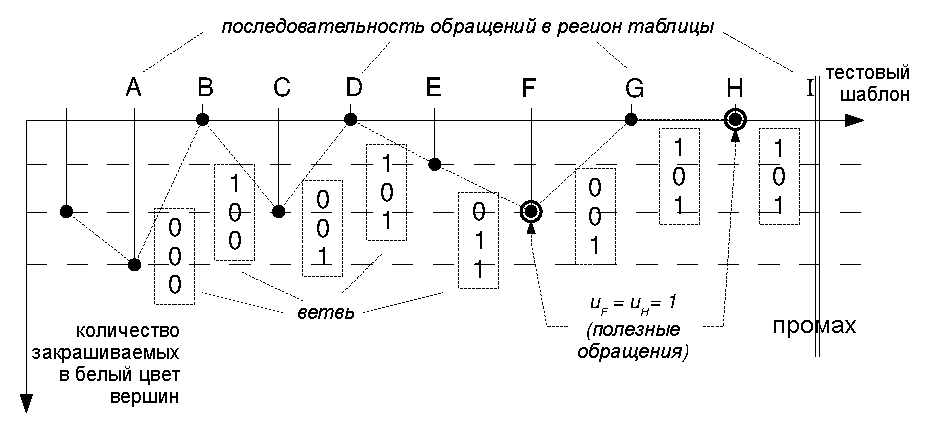
\includegraphics[width=\textwidth]{2.theor/plru_usefl_exmp}
  \caption{Перекрашивание ветви последовательностью обращений}\label{fig:plru_exmp_vytesn}
  \end{figure}

На рисунке~\ref{fig:plru_exmp_vytesn} изображен пример процесса перекрашивания для \\8-ассоциативной таблицы. В этом примере рассматривается ветвь, ведущая в строку, к которой происходит обращение А. После обращения к своей же строке вся ветвь становится белой: линия из А в В помечена (0 0 0)$^T$. Чем <<глубже>> по оси ординат происходит обращение, тем <<глубже>> становится белой ветвь (значение по оси ординат означает количество подряд вершин ветви, начиная с первой (самой верхней в векторах на рисунке), которые становятся равными нулю, а следующая за ней вершина, если она существует, становится равной единице, остальные вершины не меняются). Обращение В самое <<мелкое>>, оно лишь меняет первую вершину ветви, делая ее чёрной. Следующее обращение, С, перекрашивает 2 вершины в белый цвет (в том числе и ту вершину, которую только что обращение В покрасило в чёрный цвет) и 1 вершину в чёрный цвет. И так далее.

Обратим внимание на обращения F и H. Вершины, которые они закрашивают в чёрный цвет, сохраняют свой цвет до промаха, в котором будет определяться, вытеснять ли данную строку. Это происходит потому, что все следующие обращения происходят с закрашиванием меньшего числа вершин, чем F и H. В качестве функционала вытеснения рассмотрим количество таких обращений, как F и H, т.е. таких, после которых обращения закрашивают меньшее число вершин: самое большое число таких вершин есть длина ветви, самое малое - ноль (обращение А), изменений одной ветви определяется без отсылок к другим ветвям, вытеснение происходит тогда и только тогда, когда количество чёрных вершин равно длине ветви.

%Например, представленный на рисунке~\ref{fig:plru-useful} шаблон успевает
% покрасить 5 вершин ветви в черный цвет.
%
%\begin{figure}[t] \center
%  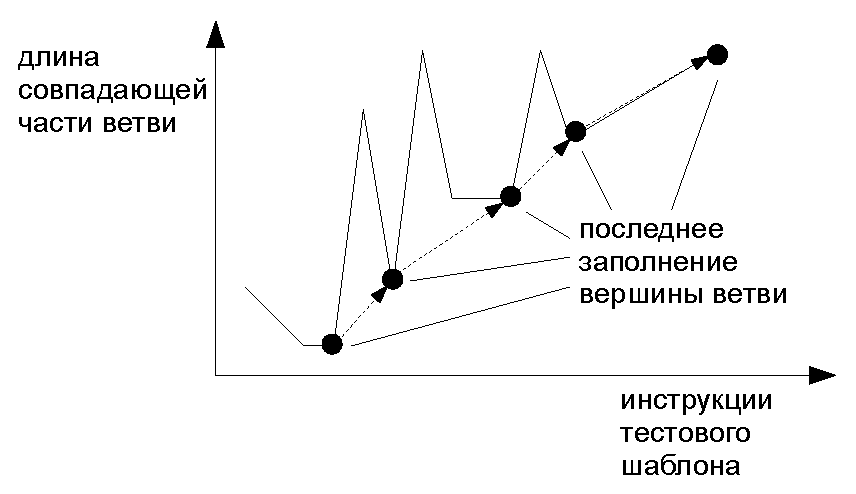
\includegraphics[width=0.6\textwidth]{2.theor/plru-useful}\\
%  \caption{Заполнение ветви черными вершинами в стратегии вытеснения
%  \PseudoLRU}\label{fig:plru-useful}
%\end{figure}

\begin{utv}
Обращение $I$ считается полезным в случае стратегии вытеснения \PseudoLRU, если все последующие обращения (до промаха, в котором вся ветвь будет чёрной) затрагивают только те вершины ветви, которые расположены выше вершины, перекрашиваемой инструкцией $I$ в черный цвет.
\end{utv}

Для вытеснения нужно не менее $\log_2 w$ полезных обращений (длина ветви). Далее выражение $\log_2 w$ будет обозначаться буквой $W$.

%Отличие этого функционала вытеснения от функционала для \LRU является \emph{немонотонность}. Это означает, что полезные инструкции надо считать для каждого промаха заново ---
%инструкции между двумя соседними промахами могут <<забелить>>
%несколько вершин ветви, что уменьшит функционал вытеснения
%(см.рис.~\ref{nonmonotonic}). Метрика для \LRU является монотонной,
%потому что инструкции между промахами не могут уменьшить функционал вытеснения -- либо не меняют, либо увеличивают ее, сдвигая ключ к концу вектора \LRU (см. рис.~\ref{monotonic}).
%
%%Таким образом, ограничение, описывающее стратегию вытеснения
%%\PseudoLRU, будет представлено дизъюнкцией ограничений по всем
%%предыдущим кэш-промахам.
%
%\begin{figure}[h] \center
%  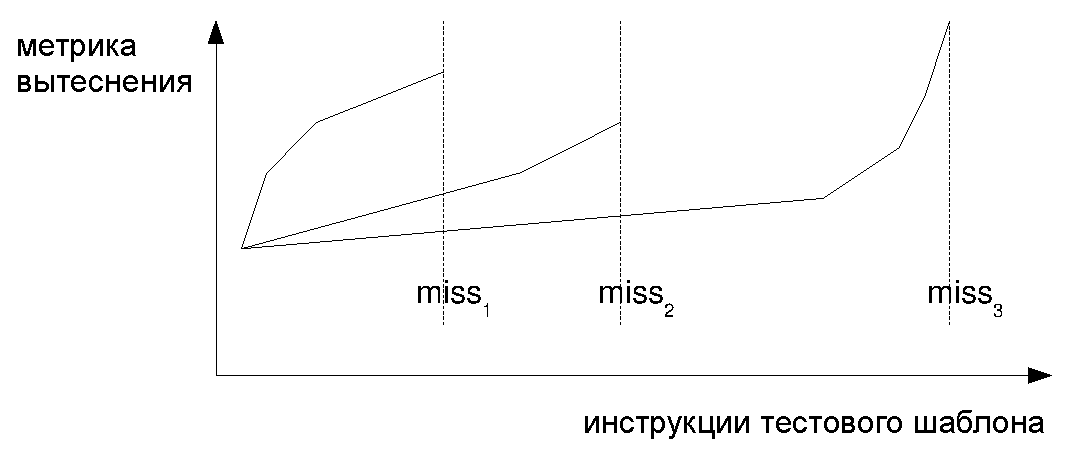
\includegraphics[width=0.6\textwidth]{2.theor/nonmonotonic}\\
%  \caption{Немонотонный функционал вытеснения}\label{nonmonotonic}
%\end{figure}
%
%\begin{figure}[h] \center
%  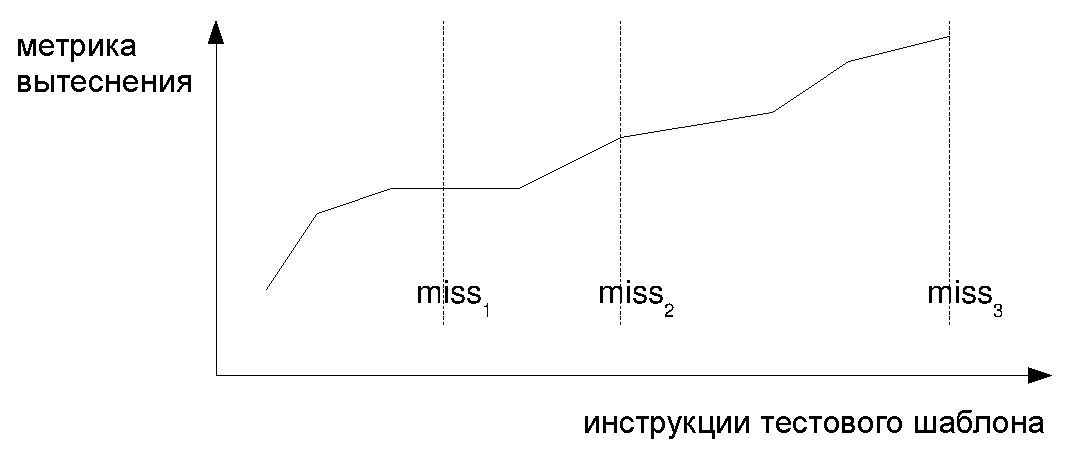
\includegraphics[width=0.6\textwidth]{2.theor/monotonic}\\
%  \caption{Монотонный функционал вытеснения}\label{monotonic}
%\end{figure}

Осталось записать формулу полезного обращения для \PseudoLRU в виде ограничений. Определимся с набором переменных. Каждому обращению в таблицу будут соответствовать следующие переменные:
\begin{itemize}
  \item ключ $k_i$;
  \item регион $R_i$;
  \item позиция $\pi_i$ (определение см. в разделе~\ref{sec:PseudoLRUonBranches}), $\pi_i \in \{0..w{-}1\}$;
  \item позиция $\pi'_i$ в момент последнего обращения перед данным (только для неинициализирующих обращений).
\end{itemize}

Обращение по ключу $k_i$ в регион $R_i$ на позицию $\pi_i$ будет полезным для вытеснения ключа $k_{n+1}$ в регионе $R_{n+1}$ ($i < n+1$) с позицией в момент последнего обращения $\pi'_{n+1}$, если выполнены все следующие условия (ниже будет доказано, что это определение соответствует стратегии вытеснения \PseudoLRU):
\begin{enumerate}
  \item <<$i$'е>> обращение происходит после последнего обращения к $k_{n+1}$ в $R_{n+1}$ перед $(n+1)$'м обращением;
  \item <<$i$'е>> обращение происходит в тот же регион, что и $R_{n+1}$;
  \item <<$i$'e>> обращение происходит до ближайшего повторного обращения на позиции $\pi'_{n+1}$;
  \item все обращения после <<$i$'го>> до ближайшего повторного обращения на позиции $\pi'_{n+1}$ просходит без закрашивания той вершины, которую красит <<$i$'e>> обращение.
\end{enumerate}

В момент последнего обращения по ключу $k_{n+1}$ в $R_{n+1}$ ветвь к нему становится целиком белой и начинается процесс вытеснения. Последующие инструкции перекрашивают эту ветвь до тех пор, пока не встретится обращение с промахом на той же позиции, которая была в момент последнего обращения к $k_{n+1}$ в $R_{n+1}$. К этому моменту вся ветвь должна стать чёрной, а после этого обращения ветвь вновь становится белой, но эта ветвь уже относится к другому ключу (тому, который вытеснил $k_{n+1}$).

Поясню этот момент с другой стороны. Рассматривая успешность очередного обращения к некоторому ключу, ищем ближайшее предыдущее обращение к тому же ключу (обращение А на рисунке~\ref{fig:plru_exmp_vytesn}). Обращения, идущие после этого <<предыдущего>>, либо должны вытеснить соответствующий ключ (если речь идёт о неуспешном обращении), либо не должны вытеснить (если --- об успешном). Если среди этих обращений не встречается обращение по той же позиции, что и в момент <<предыдущего>> обращения, то вытеснение не произойдет (т.к. в противном случае в этом обращении могло произойти бы вытеснение по определению \PseudoLRU). Если же обращение встречается (обращение I на рисунке~\ref{fig:plru_exmp_vytesn}), то к его моменту вся ветвь должна успеть стать полностью чёрной.

Переменные $\pi_i$ для позиций обладают собственными ограничениями, не зависящими от успешности обращений по ним. А именно, позиции --- это битовые строки длины $W$, идентифицирующие ключи: если позиции двух обращений совпадают и между ними нет промахов по этой позиции, то ключи должны совпадать, если же позиции различаются, то и ключи должны различаться (обозначим $t_i$ и $r_i$ --- ключи и регионы инициализирующих обращений, $k_i$ и $R_i$ --- ключи и регионы в обращениях из тестового шаблона, обозначим $s \equiv \langle (t_1||r_1), ..., (t_m||r_m), (k_1||R_1), ..., (k_n||R_n)\rangle$):

для каждой пары обращений $i$ и $j$ ($j$'е --- после $i$'го)
\begin{itemize}
    \item если $S_j$ = hit, то $$(\pi_i||R(s_i) = \pi_j||R(s_j)~\wedge$$ $$\pi_i||R(s_i) \notin \{\pi_{m_1}||R(s_{m_1}), \pi_{m_2}||R(s_{m_2}), \dots, \pi_{m_n}||R(s_{m_n})\}) \rightarrow s_i = s_j$$
    \item если $S_j$ = miss, то $$(\pi_i||R(s_i) = \pi_j||R(s_j)~\wedge$$ $$\pi_i||R(s_i) \notin \{\pi_{m_1}||R(s_{m_1}), \pi_{m_2}||R(s_{m_2}), \dots, \pi_{m_n}||R(s_{m_n})\}) \rightarrow s_i \neq s_j$$
\end{itemize}
где $(\pi_{m_1},R(s_{m_1})), (\pi_{m_2},R(s_{m_2})), \dots, (\pi_{m_n},R(s_{m_n}))$ --- позиции и регионы неуспешных обращений,
расположенных между $i$'м и $j$'м обращениями. В качестве $i$'го обращения также надо рассмотреть и инициализирующие обращения.

%% это "перевернутые"позиции! у них чем ближе к листу, тем дальше от левой границы в битовом представлении

И, наконец, определение для $\pi'_i$ в виде ограничений. Если $S_i$ = hit, то  $\pi'_i$ --- позиция в том обращении, где в последний раз встретился ключ $k_i$ в регионе $R_i$:
$$
\begin{array}{l}
\texttt{(ite~} ((k_i||R_i) = (k_{i-1}||R_{i-1})) ~~ (\pi'_i = \pi_{i-1})\\
\texttt{(ite~} ((k_i||R_i) = (k_{i-2}||R_{i-2})) ~~ (\pi'_i = \pi_{i-2})\\
... ~(\pi'_i = 0)\texttt{)))...)}\\
\end{array}
$$

Подформула $\pi'_i = 0$ не оказывает влияния, если $(k_i||R_i) \in \{(k_{i-1}||R_{i-1}),$ $(k_{i-2}||R_{i-2}), ... \}$, а так и будет

Если $S_i = $ miss, то кроме того, что $\pi'_i$ --- позиция последнего вхождения ключа $k_i$ в регионе $R_i$, надо убедиться, что та же позиция $\pi'_i$ встречается после последнего обращения к $k_i$ в $R_i$ на неуспешном обращении ( $\{\pi_i, ..., \pi_j\}_m$ обозначает подмножество множества позиций от $i$'го до $j$'го обращения из неуспешных обращений):
$$
\begin{array}{l}
\texttt{(ite~} ((k_i||R_i) = (k_{i-1}||R_{i-1})) ~~ (\pi'_i = \pi_{i-1})\\
\texttt{(ite~} ((k_i||R_i) = (k_{i-2}||R_{i-2})) ~~ (\pi'_i = \pi_{i-2} \wedge \pi'_i \in \{\pi_{i-1}\}_m)\\
\texttt{(ite~} ((k_i||R_i) = (k_{i-3}||R_{i-3})) ~~ (\pi'_i = \pi_{i-3} \wedge \pi'_i \in \{\pi_{i-1}, \pi_{i-2}\}_m)\\
... ~(\pi'_i = 0)\texttt{)))...)}\\
\end{array}
$$

Переходим непосредственно к записи формулы полезного обращения. Запишем каждое условие этого определения в виде ограничений ( $k_{n+1}$ и $R_{n+1}$ --- ключ и регион, по отношению к которым определяется вытеснение, $s \equiv \langle (t_1||r_1), ..., (t_m||r_m), (k_1||R_1), ..., (k_n||R_n)\rangle$ --- предыдущие обращения (ключи и регионы), $\sigma \equiv \langle (\tau_1||r_1), ..., (\tau_m||r_m), (\pi_1||R_1), ..., (\pi_n||R_n)\rangle$ --- предыдущие обращения (позиции и регионы), $i$ --- номер обращения, для которого записывается формула полезного обращения, $R(s_i)$ --- вторая компонента $s_i$, $R(\sigma_i)$ --- вторая компонента $\sigma_i$, $\pi(\sigma_i)$ --- первая компонента $\sigma_i$) :
\begin{enumerate}
    \item $(k_{n+1}||R_{n+1}) \notin \{s_i, s_{i+1}, ...,  s_{m+n}\}$ -- $i$'е обращение происходит после последнего обращения к $k_{n+1}$ в $R_{n+1}$;
    \item $R_{n+1} = R(s_i)$ -- обращение происходит в тот же регион;
    \item $(\pi'_{n+1}||R_{n+1}) \in \{\sigma_i, \sigma_{i+1}, ..., \sigma_{m+n}\}$ -- обращение происходит до ближайшего повторного обращения на ту же позицию;
    \item $\bigwedge\limits_{j = i+1}^n (((\pi'_{n+1}||R_{n+1}) \notin \{\sigma_i, \sigma_{i+1}, ..., \sigma_j\}~\wedge~R(\sigma_i) = R(\sigma_j)) \rightarrow P(\pi(\sigma_i) \oplus \pi'_{n+1}, \pi(\sigma_j) \oplus \pi'_{n+1}))$ --- полезные инструкции должны закрашивать больше белых вершин, чем закрашивают все последующие инструкции;  предикат $P$ для пары векторов $\delta_i$ и $\delta_j$ (<<относительных позиций>> --- см. раздел~\ref{sec:PseudoLRUonBranches}) истинен тогда и только тогда, когда количество старших нулевых бит у $\delta_i$ больше количества старших нулевых бит у $\delta_j$, иными словами, только и только тогда, когда существует целое $k$ такое, что $\delta_i < 2^k \leqslant \delta_j$ (см.рис.~\ref{fig:bits}); из леммы~\ref{QuantorElimination} (ее формулировка и доказательство находятся в приложении~\ref{sec:proofs}) следует, что этот предикат обладает бескванторной эквивалентной формой: $P(\delta_i, \delta_j) \equiv (\delta_j > \delta_i~~\wedge~~\delta_j \oplus \delta_i > \delta_i)$, сравнения беззнаковые.
\end{enumerate}

\begin{figure}[h] \center
  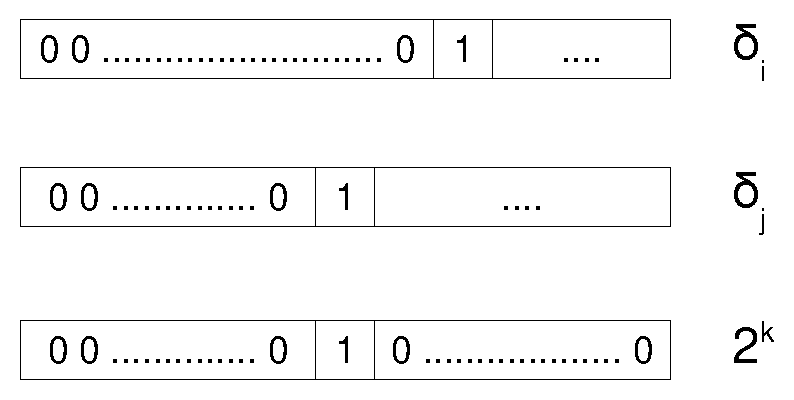
\includegraphics[width=0.4\textwidth]{2.theor/bits}\\
  \caption{Перекрашивание и битовые строки}\label{fig:bits}
\end{figure}

Итак, система ограничений для описания обращений по ключу $k_i$ в регион $R_i$ согласно методу полезных обращений для \PseudoLRU:
\begin{itemize}
\item для hit($k_i, R_i$):
$$
\left\{\begin{array}{l}
(k_i||R_i) \in \{(t_1||r_1), ..., (t_m||r_m), (k_1||R_1), ..., (k_{i-1}||R_{i-1})\}\\
\{(t_1||r_1), ..., (t_m||r_m)\} - \mbox{все разные}\\
\sum\limits_{j=1}^m [u_{k_i,R_i,\pi'_i}(t_j||r_j)] + \sum\limits_{j=1}^{i-1} [u_{k_i,R_i,\pi'_i}(k_j||R_j)] < W\\
\end{array} \right.
$$
\item для miss($k_i, R_i$):
$$
\left\{\begin{array}{l}
(k_i||R_i) \in \{(t_1||r_1), ..., (t_m||r_m), (k_1||R_1), ..., (k_{i-1}||R_{i-1})\}\\
\{(t_1||r_1), ..., (t_m||r_m)\} - \mbox{все разные}\\
\sum\limits_{j=1}^m [u_{k_i,R_i,\pi'_i}(t_j||r_j)] + \sum\limits_{j=1}^{i-1} [u_{k_i,R_i,\pi'_i}(k_j||R_j)] \geqslant W\\
\end{array} \right.
$$
\end{itemize}

$$u_{k_i,R_i,\pi'_i} (s_j)  \equiv \left\{\begin{array}{l}
(k_i||R_i) \notin \{s_j, s_{j+1}, ..., s_{m+n}\}\\
R_i = R(s_j)\\
(\pi'_i||R_i) \in \{(\pi_j||R_j), (\pi_{j+1} || R_{j+1}), ..., (\pi_{m+n}||R_{m+n})\}\\
\bigwedge\limits_{l = j+1}^{m+n} (R_j = R_l ~\wedge~(\pi'_i||R_i) \notin \{(\pi_j||R_j), (\pi_{j+1}||R_{j+1}), ..., (\pi_l||R_l)\}\\
 \hspace{2cm} \rightarrow P(\pi_j \oplus \pi'_i, \pi_l \oplus \pi'_i))\\
\end{array}\right.
$$
$$s \equiv \langle (t_1,r_1), (t_2,r_2), ..., (t_m,r_m), (k_1, R_1), ..., (k_n,R_n) \rangle$$
$$R(s_i) \mbox{~--- вторая компонента~} s_i$$
$$P(x, y) \equiv (y > x~~\wedge~~x \oplus y > x)$$


%Таблица~\ref{plru_table} содержит ограничения для разных случаев
%кэш-попаданий и кэш-промахов (см. утверждение~\ref{hit_miss_human}).
%В каждое из них включается ограничение на количество полезных
%инструкций согласно предлагаемой методике использования функций
%полезности. Полезности считаются относительно некоторого кэш-промаха
%(для их перебора используется сокращение $x_m : \mbox{miss}$).

В приложении~\ref{sec:proofs} доказана теорема~\ref{PLRUusefulThm} эквивалентности этих формул определению стратегии вытеснения \PseudoLRU.

Немного изменив формулу для $\pi'_i$, можно упростить ограничения \textbf{для}\\ \textbf{успешных} обращений. А именно, определив $\pi'_i$ так:

$$
\begin{array}{l}
\texttt{(ite~} (s_i = s_{i-1}) ~~ (\pi'_i = \pi_{i-1})\\
\texttt{(ite~} (s_i = s_{i-2}) ~~ (\pi'_i = \pi_{i-2} \wedge \pi'_i \neq \pi_{i-1})\\
...\\
\texttt{(ite~} (s_i = s_j) ~~ (\pi'_i = \pi_j \wedge \pi'_i \notin \{\pi_{j+1}, ..., \pi_{i-1}\})\\
... \texttt{~true )))...)}\\
\end{array}
$$

для hit($k_i, R_i$) будет достаточно таких ограничений:
$$
\left\{\begin{array}{l}
(k_i||R_i) \in \{(t_1||r_1), ..., (t_m||r_m), (k_1||R_1), ..., (k_{i-1}||R_{i-1})\}\\
\{(t_1||r_1), ..., (t_m||r_m)\} - \mbox{все разные}\\
\end{array} \right.
$$
т.е. ограничение на сумму будет автоматически выполнено. Этот факт следует из того, что о возможности вытеснения можно вести речь там, где встречается хотя бы одно неуспешное обращение на позиции $\pi'_i$. Если же позиция $\pi'_i$ не встречается после последнего обращения к ключу $k_i$, то и вытеснение произведено не будет (в формулах полезных обращений третье условие ложно для всех $s_j$, значит, количество полезных обращений равно равно 0, что означает невытеснение).

\subsection{Разрешение ограничений, описывающих стратегии вытеснения}

Ограничения, которые предлагается строить для описания количества полезных обращений, являются \emph{ограничениями мощности} (cardinality constraints). Это
ограничения вида $C_1 \leqslant \sum_{i=1}^n a_i \leqslant C_2$, где $C_1, C_2$
-- неотрицательные целые числа, а $a_i$ принимают значения 0 или
1~\cite{smt_debugging, PiskacK08, KuncakR07,
Revesz05}. Речь идет об ограничении размера некоторого множества
элементов, заданного с помощью характеристической функции.
В~\cite{smt_debugging} проведено исследование способов записи
ограничений мощности и показано, что от формы записи зависит
эффективность разрешения этих ограничений. Одна из таких форм рассматривает ограничения
мощности как компактную форму записи уравнения
вида $\bigvee_{C_1 \leqslant C \leqslant C_2} \sum_{i=1}^n a_i = C$,
где равенство есть
\begin{itemize}
\item тождественная ложь, если $C < 0$ или $C > n$;
\item конъюнкция $\bigwedge_{1\leqslant i\leqslant n} (a_i = 0)$,
если $C = 0$;
\item дизъюнкция по всевозможным выборкам индексов $i_1, ..., i_C$, где
для каждого индекса $i_k$ справедливы свойства $1 \leqslant i_k
\leqslant n$ и $i_k < i_{k+1}$, конъюнкций $\bigwedge_{i_k} (a_{i_k}
= 1)$, если $1 \leqslant C \leqslant n$.
\end{itemize}

В диссертации не ставилась задача исследования способов разрешения ограничений
мощности (с целью выбора наиболее эффективного способа их представления). Вместо
этого были использованы
имеющиеся инструменты разрешения ограничений мощности~\cite{Z3, Yices}. Для
записи оставшихся формул был использован язык битовых строк, для разрешения
ограничений над которым существуют эффективные SMT-инструменты (например,
Z3~\cite{Z3}).

%После устранения ограничений мощности в формуле остаются только
%ограничения на конечные множества тегсетов: принадлежности и
%непринадлежности тега конечному множеству тегсетов и равенства и
%неравенства битовых полей тегсетов. Поскольку конечные множества
%тегсетов известны (заданы перечислением тегсетов, которые в входят в
%это множество), то ограничения принадлежности и непринадлежности
%могут быть переписаны без использования этих отношений. Отношение
%принадлежности $x \in \{x_1, x_2, ..., x_n\}$ может быть переписано
%в виде дизъюнкции $(x = x_1) \vee (x = x_2) \vee ... \vee (x =
%x_n)$, а отношение непринадлежности $x \notin \{x_1, x_2, ...,
%x_n\}$ -- в виде конъюнкции $(x \neq x_1) \wedge (x \neq x_2) \wedge
%... \wedge (x \neq x_n)$.
%
%В результате получается предикат, в котором переменными величинами
%являются неотрицательные целые числа с конечной областью значений
%(тегсеты), над переменными возможны операции получения битового
%поля, в предикате используется отношение равенства и неравенства над
%битовыми полями. Кроме того, этот предикат задается с использованием
%ограничений мощности.
%
%Для разрешения такого рода предикатов можно было бы разрабатывать
%собственные процедуры распространения ограничений, но это свело бы
%на нет все усилия по выработке собственного представления стратегии
%вытеснения. Однако предлагаемые ограничения могут быть тривиальным
%образом выражены на языке теорий, для которых существуют эффективные
%разрешающие процедуры (битовые строки, неинтерпретируемые функции).
%Поэтому для записи и разрешения этих ограничений могут быть
%использованы SMT-инструменты~\cite{Z3}.

%%%%%%%%%%%%%%%%%%%%%%%%%%%%%%%%%%%%%%%%%%%%%%%%%%%%%%%%%%%%%%%%%%%
%
%\pagebreak
%\section{Ограничения, описывающие тестовые ситуации в некоторых
%частных случаях, для стратегии вытеснения \LRU}
%
%\subsection{Тестовые шаблоны без кэш-промахов}
%
%В случае тестовых шаблонов, в которых нет кэш-промахов, нет ни
%вытесняющих, ни вытесняемых тегсетов. Поэтому в таких шаблонов
%уравнения для кэш-попаданий имеют очень простой вид:
%
%$$
%\left\{
%\begin{array}{l}
%x \in D\\
%... (\mbox{тестовые ситуации на остальные буферы})\\
%\end{array}
%\right.
%$$
%
%\subsection{Тестовые шаблоны без кэш-попаданий}
%
%В случае тестовых шаблонов, в которых нет кэш-попаданий, надо
%генерировать ограничения для вытесняющих и лишь иногда для
%вытесняемых тегсетов. А именно, вытесняемый тегсет требуется лишь в
%том случае, когда кэш-промах вносит в кэширующий буфер ранее
%вытесненный тегсет. В этом случае для вытесняемого тегсета известен
%домен, что позволяет построить уравнения обозримого размера. Кроме
%того, поскольку отсутствуют кэш-попадания, повторные обращения к
%вытесняемым тегсетам (кроме кэш-промаха, который их может внести в
%кэширующий буфер) невозможны, что также упрощает генерируемые
%уравнения.
%
%В результате получается, что вытесняющий тегсет описывается в
%тестовом шаблоне без кэш-попаданий следующей системой уравнений:
%$$
%F'(x) \vee F''(x) \vee \bigvee_{\lambda_\delta \in D} F'''(x, \lambda_\delta)
%$$
%
%где
%
%$$F'(x) \equiv (x \notin D \wedge x \notin \{x_1, ..., x_n\})$$
%
%$$F''(x) \equiv (x \in \{x_1, ..., x_n\} \wedge \sum_{i=1}^n u''(x_i) \geqslant w)$$
%
%$$u''(x_i) \equiv (x\notin \{x_i, ..., x_n\} \wedge R(x_i) = R(x))$$
%
%$$F'''(x, \lambda_\delta) \equiv (x = \lambda_\delta \wedge x \notin
%\{x_1, ..., x_n\} \wedge \sum_{i=1}^n (R(x_i) = R(x)) \geqslant w -
%\delta + 1)$$
%
%\subsection{Короткие тестовые шаблоны}
%
%Будем называть тестовый шаблон \emph{коротким}, если в нем не более
%$w$ инструкций обращения к памяти. Очевидно, что любой короткий
%тестовый шаблон является простым. Из 7 случаев для коротких тестовых
%шаблонов остается всего 5 (первые два можно еще объединить в более
%компактную систему уравнений). В таблице~\ref{short_templates_table}
%предъявлены функции полезности и ограничения для коротких тестовых
%шаблонов в случае стратегии вытеснения \LRU. Соответствующая теорема
%корректности этих ограничений сформулирована и доказана в
% приложении~\ref{sec:proofs}.
%
%\begin{table}[t]
%\begin{tabular}{|c|c|c|c|}
%\hline  & \centering случай &
%\begin{tabular}{c}переменная\\перебора\end{tabular} & система \\
%\hline \hline \multirow{-2}{*}{\rotatebox{90}{кэш-попадание}} &
%\makecell[c{p{0.3\textwidth}}]{тегсет находится в начальном
%состоянии буфера и он всё ещё не вытеснен} & $\lambda_\delta \in D$
%&
%$\left\{\begin{array}{l} x = \lambda_\delta\\
%\sum\limits^n_{i=1} u(x_i) \leqslant w - \delta
%\end{array}\right.$ \\ \hhline{~|---}
%& \makecell[c{p{0.3\textwidth}}]{тегсет уже встречался в шаблоне} &
%-- & $x \in \{x_1, ..., x_n\}$
%\\ \hline \hline \multirow{6}{*}{\rotatebox{90}{кэш-промах}}
%& \makecell[c{p{0.3\textwidth}}]{тегсет встречается впервые} & -- &
%$\left\{\begin{array}{l} x \notin D\\
%x \notin \{x_1, ..., x_n\}\\
%\end{array}\right.$\\ \hhline{~|---} &
%\makecell[c{p{0.3\textwidth}}]{тегсет находился в начальном
%состоянии буфера и был вытеснен} & $\begin{array}{c}\lambda_\delta
%\in D,\\\delta \geqslant w-n+1\end{array}$ &
%$\left\{\begin{array}{l} x = \lambda_\delta\\
%x \notin \{x_1, ..., x_n\}\\
%\sum\limits^n_{i=1} u(x_i) > w - \delta\\
%\end{array}\right.
%$ \\ \hline
%\end{tabular}
%
%%где функция полезности определена следующим образом:
%$$u(x_i) \equiv
%\left\{\begin{array}{l} x_i \in \{ \lambda_{\delta+1}, ...,
%\lambda_w\}~\wedge~x_i \notin \{x_1, ..., x_{i-1}\}, \mbox{если}~S_i
%= \mbox{hit}\\
%R(x_i) = R(x), \mbox{если}~S_i = \mbox{miss}
%\end{array}\right.
%$$
%\caption{Таблица систем уравнений для тестовых ситуаций в кэширующих
%буферах для коротких тестовых шаблонов в случае стратегии вытеснения
%\LRU}\label{short_templates_table}
%\end{table}
%
%
%
%%\begin{landscape}
%%\begin{table}
%%\begin{tabular}{|c|c|c|c|c|c|}
%%\hline  & \centering случай &
%%\begin{tabular}{c}переменная\\перебора\end{tabular} & система &
%%\begin{tabular}{c}функция\\полезности\\для кэш-\\попадания\end{tabular} &
%%\begin{tabular}{c}функция\\полезности\\для кэш-\\промаха\end{tabular} \\
%%\hline \hline \multirow{-2}{*}{\rotatebox{90}{кэш-попадание}} &
%%\makecell[c{p{0.3\textwidth}}]{тегсет находится в начальном
%%состоянии буфера и он всё ещё не вытеснен} & $\lambda_\delta \in
%%D$ &
%%$\left\{\begin{array}{l} x = \lambda_\delta\\
%%\sum\limits^n_{i=1} u(x_i) \leqslant w - \delta
%%\end{array}\right.
%%$ &
%%\begin{tabular}{c}
%%$x_i \in \{ \lambda_{\delta+1}, ..., \lambda_w\}$\\
%%$\wedge~x_i \notin \{x_1, ..., x_{i-1}\}$
%%\end{tabular}
%%& $R(x_i) = R(x)$
%%\\ \hhline{~|-----}
%%& \makecell[c{p{0.3\textwidth}}]{тегсет уже встречался в шаблоне} &
%%-- & $x \in \{x_1, ..., x_n\}$ & -- & --
%%\\ \hline \hline \multirow{6}{*}{\rotatebox{90}{кэш-промах}}
%%& \makecell[c{p{0.3\textwidth}}]{тегсет встречается впервые} & -- &
%%$\left\{\begin{array}{l} x \notin D\\
%%x \notin \{x_1, ..., x_n\}\\
%%\end{array}\right.
%%$ & -- & -- \\ \hhline{~|-----} &
%%\makecell[c{p{0.3\textwidth}}]{тегсет находился в начальном
%%состоянии буфера и был вытеснен} &
%%$\begin{array}{c}\lambda_\delta \in D,\\\delta \geqslant
%%w-n+1\end{array}$ &
%%$\left\{\begin{array}{l} x = \lambda_\delta\\
%%x \notin \{x_1, ..., x_n\}\\
%%\sum\limits^n_{i=1} u(x_i) > w - \delta\\
%%\end{array}\right.
%%$ &
%%\begin{tabular}{c}
%%$x_i \in\{\lambda_{\delta+1}, ..., \lambda_w\}$\\
%%$\wedge~x \notin \{x_1, ..., x_{i-1}\}$\\
%%\end{tabular}
%%&
%%\begin{tabular}{c}
%%$R(x_i) = R(x)$\\
%%\end{tabular}
%%\\ \hline
%%\end{tabular}
%%\caption{Таблица систем уравнений для тестовых ситуаций в кэширующем буфере
%%для коротких тестовых шаблонов в случае стратегии вытеснения
%%\LRU}\label{short_templates_table}
%%\end{table}
%%\end{landscape}
%
%
%\subsection{Генерация тестовых данных для кэш-памяти, содержащей
%<<грязные>> ячейки}
%
%Любая ячейка в кэш-памяти может быть помечена \emph{грязной}
%(\emph{invalid}). Это означает, что данные, находящиеся в кэширующем
%буфере по этому адресу, не могут использоваться в качестве данных,
%хранящихся в памяти по этому адресу.
%
%Рассмотренные ранее в этой работе случаи не учитывали грязные ячейки
%кэширующем буфере, хотя они зачастую присутствуют в микропроцессоре
%после его запуска -- с таким состоянием кэширующего буфера работают
%первые после запуска микропроцессора инструкции.
%
%Кэш-попадание возникает в том случае, когда требуемые данные
%присутствуют среди <<чистых>> ячеек кэширующего буфера. Кэш-промах
%возникает в том случае, когда требуемых данных нет среди <<чистых>>
%ячеек. Причем при наличии <<грязных>> ячеек вытеснения может и не
%произойти. А именно, если все ячейки набора, с которым работает
%инструкция, являются <<чистыми>>, то происходит вытеснение согласно
%стратегии вытеснения, остальные наборы не меняются. Если же среди
%ячеек набор есть <<грязные>> ячейки, то вытеснение не происходит, а
%на место одной из <<грязных>> ячеек помещаются данные из основной
%памяти по заданному адресу и ячейка объявляется <<чистой>>.
%Остальные ячейки не меняются. В стратегии вытеснения \LRU эта бывшая
%<<грязная>> ячейка становится самой новой.
%
%Для генерации тестовых данных для кэширующих буферов с грязными
%ячейками предлагается применять ограничения с функциями полезности.
%Примечательно, что наличие грязных ячеек не меняет качественно
%систему уравнений.
%
%В данном разделе рассматривается случай, когда начальное состояние
%микропроцессора известно. Кроме того, рассматриваемый случай
%учитывает отсутствие инструкций в тестовом шаблоне, которые
%превращали бы <<чистые>> ячейки в <<грязные>> (т.е. все такие
%изменения должны делаться явно вне тестовых шаблонов).
%
%\subsubsection{случай полностью-ассоциативного кэширующего буфера}
%
%В случае полностью-ассоциативных кэширующих буферов очевидно, что
%первые кэш-промахи будут заполнять <<грязные>> ячейки. Пусть $N$ --
%количество <<грязных>> ячеек в начальном состоянии кэширующего
%буфера, а $L_0$ -- начальное состояние (выражение) кэширующего
%буфера (только <<чистые>> ячейки). Тогда для тестовых ситуаций надо
%генерировать такие ограничения ($L$ -- выражение для состояния
%кэширующего буфера перед исполнением инструкции, $L'$ -- выражение
%для состояния кэширующего буфера после исполнения инструкции):
%\begin{itemize}
%\item для \emph{кэш-попадания} hit($x$) генерируются ограничения
%$$
%\left\{
%\begin{array}{l}
%x \in L\\
%L' \equiv L\\
%\end{array}
%\right.
%$$
%
%\item для \emph{кэш-промаха} miss($x$), если это один из первых $N$
%кэш-промахов, генерируются ограничения:
%$$
%\left\{
%\begin{array}{l}
%x \notin L\\
%L' \equiv L \cup \{x\}\\
%\end{array}
%\right.
%$$
%
%\item для \emph{кэш-промаха} miss($x$), являющегося по счету более
%чем $N$'м кэш-промахом тестового шаблона, генерируются ограничения:
%$$
%\left\{
%\begin{array}{l}
%x \notin L\\
%x' \in L\\
%L' \equiv L\setminus\{x'\} \cup \{x\}\\
%displaced(x', L)\\
%\end{array}
%\right.
%$$
%\end{itemize}
%
%Предикат $displaced(x', L)$ истинен, если $x'$ является вытесняемым
%тегом в текущем состоянии кэширующего буфера $L$. Для стратегии
%вытеснения \LRU этот предикат может быть записан с использованием
%тех же диапазонов вытеснения, что и для кэширующего буфера без
%<<грязных>> ячеек (см.п.~\ref{LRU_constraints}). А именно, диапазон
%вытеснения начинается на инструкции, которая последний раз перед
%вытеснением тега обращается к нему. Тогда между этой инструкцией и
%инструкцией, вытесняющей $x$, должны быть обращения ко всем
%остальным тегам текущего состояния кэширующего буфера. Эта логика
%может быть записана в виде тех же уравнений, что и в
%пункте~\ref{LRU_constraints}. Нетрудно проверить, что для
%кэширующего буфера с <<грязными>> ячейками остается справедливой
%лемма о невложенных диапазонах вытеснения, что доказывает
%корректность использования ограничений из
%пункта~\ref{LRU_constraints} для кэширующего буфера с <<грязными>>
%ячейками.
%
%\subsubsection{случай наборно-ассоциативного кэширующего буфера}
%
%В этом пункте будет показано, что ограничения для кэширующего
%буфера, начальное состояние которого содержит <<грязные>> ячейки,
%качественно не отличаются от ограничений для кэширующего буфера без
%<<грязных>> ячеек.
%
%Аналогично тому, как это делалось для кэширующих буферов без
%<<грязных>> ячеек, для тестовых ситуаций на кэширующие буферы с
%<<грязными>> ячейками тоже возможно следующее исчерпывающее
%выделение случаев:
%\begin{itemize}
%\item кэш-попадание тега:
%    \begin{enumerate}
%    \item данный тег находился в начальном состоянии кэширующего буфера и не был
%    вытеснен к моменту данной инструкции;
%    \item данный тег был внесен в кэширующий буфер одной из инструкций
%    кэш-промаха и с тех пор не был вытеснен;
%    \end{enumerate}
%\item кэш-промах тега:
%    \begin{enumerate}
%    \item данный тег не встречался ранее (не находился в начальном
%    состоянии кэширующего буфера и не был внесен какими-либо кэш-промахами);
%    \item данный тег был ранее вытеснен из кэширующего буфера и с тех пор
%    не был внесен в кэширующий буфер вновь.
%    \end{enumerate}
%\end{itemize}
%
%Соответствующие ограничения приведены в
%таблице~\ref{dirty_hit_miss_table}.
%
%
%В таблице~\ref{dirty_hit_miss_table} символ $\Delta$ означает
%количество <<чистых>> ячеек в начальном состоянии того региона, про
%который идет речь в уравнении. На самом деле $\Delta$ есть функция
%региона ($\Delta = \Delta(\lambda_\delta)$), но для сокращения
%записи оставлен только функциональный символ. Кроме того, в
%приведенных уравнениях домен переменной включает только <<чистые>>
%ячейки.
%
%Сходства уравнений (со случаем кэширующих буферов без <<грязных>>
%ячеек) удалось добиться за счет рассмотрения <<грязных>> ячеек, как
%ячеек с наименьшим счетчиком \LRU, которые не участвуют в
%определении нахождения тега в кэширующих буферах. Поэтому в функциях
%полезности участвуют множества не $\{\lambda_{\delta+1}, ...,
%\lambda_w\}$, а множества $\{\lambda_{\delta+1}, ...,
%\lambda_\Delta\}$. Все <<чистые>> ячейки получили первые индексы,
%т.е. индексы всех от 1 до $\Delta$.
%
%%\begin{theorem}[корректность использования функций полезности для
%%записи \LRU в случае наличия <<грязных>> ячеек в начальном состоянии
%%кэширующего буфера] Тестовая программа, построенная по ограничениям,
%%которые сгенерированы с использованием предъявленных в
%%таблице~\ref{dirty_hit_miss_table} функций полезности, в случае
%%наличия <<грязных>> ячеек в начальном состоянии кэширующего буфера
%%удовлетворяет своему тестовому шаблону.
%%\end{theorem}
%%\begin{proof}
%%  //TODO
%%\end{proof}
%
%Для приведенных ограничений также могут быть применены эвристики,
%сокращающие их количество, которые были упомянуты для кэширующих
%буферов без <<грязных>> ячеек. Кроме того, в данном случае возможна
%дополнительная эвристика \emph{ограничение на $\delta$}: если
%$\delta + 1 < \Delta$, то функция полезности, в которую входит
%множество $\{\lambda_{\delta+1}, ..., \lambda_\Delta\}$, равна 0.
%
%%\subsection{Функции полезности для зеркальной генерации тестовых
%%данных}
%%
%%Рассмотрим ограничения, генерируемые для тестовых шаблонов
%%зеркальным методом с использованием функций полезности. По сравнению
%%с представленными ограничениями (см. табл.~\ref{hit_miss_table})
%%зеркальная генерация имеет свои особенности:
%%\begin{enumerate}
%%  \item множества констант (как, например, $L, D$) не используются,
%%  поэтому в ограничениях будут отсутствовать соответствующие им
%%  случаи;
%%  \item так как теги инструкций тестового шаблона должны появиться
%%  среди инициализирующей последовательности, то для вытеснения
%%  требуется $w-1$ инструкций, где $w$ -- ассоциативность кэширующего буфера;
%%  \item учет полезных инструкций начинается уже в инициализирующей
%%  последовательности, тем самым необходимо сформулировать функцию
%%  полезности для инициализирующих инструкций.
%%\end{enumerate}
%%
%%Следующая теорема описывает функцию полезности для инициализирующих
%%инструкций и описывает ограничения, генерируемые для тестовых
%%шаблонов зеркальным методом с использованием функций полезности
%%(количество инициализирующих инструкций зафиксировано, оно будет
%%обозначено параметром $m$):
%%
%%\begin{theorem}[Корректность ограничений, генерируемые зеркальным методом с
%%использованием функций полезности для
%%\LRU]\label{correct_mirror_LRU} Пусть $t_1, t_2, ..., t_m$ -- теги
%%инициализирующей последовательности, $x$ -- текущий тег тестового
%%шаблона, $x_1, x_2, ..., x_n$ -- теги предыдущих инструкций
%%тестового шаблона, причем $x \in \{t_1, ..., t_m, x_1, ..., x_n\}$ и
%%$\{t_1, ..., t_m\}$ --- все разные. Тогда $x$ не вытеснен согласно
%%определению на списках тогда и только тогда, когда
%%$$\sum\limits_{i=1}^{m+n} u_x(s_i) < w$$
%%где последовательность $s \equiv \langle t_1, ..., t_m, x_1, ...,
%%x_n\rangle$, а функция полезности определена следующим образом:
%%$$u_x(s_i) \equiv (x \notin \{s_i, ..., s_{m+n}\} \wedge
%%R(x) = R(s_i) \wedge s_i \notin\{s_{i+1},..., s_{m+n}\})$$
%%
%%%$$\sum\limits_{i=1}^m \tilde{u}_x(t_i) + \sum\limits_{i=1}^n u_x(x_i) < w$$
%%%где функции полезности определены следующим образом:
%%%$$\begin{array}{c}
%%%\tilde{u}_x(t_i) \equiv (x \notin \{t_i, ..., t_m, x_1, ..., x_n\}
%%%\wedge R(x) = R(t_i))\\u_x(x_i) \equiv (x \notin \{x_i, ..., x_n\}
%%%\wedge R(x) = R(x_i))\end{array}$$
%%
%%%$$\begin{array}{c}u_x(x_i) \equiv (x \notin \{x_i, ..., x_n\} \wedge R(x) =
%%%R(x_i)), \mbox{если}~S_i=\mbox{miss}\end{array}$$
%%%$$\begin{array}{c}u_x(x_i) \equiv (x \notin \{x_i, ..., x_n\} \wedge R(x) =
%%%R(x_i) \wedge \sum\limits_{j=1}^{m} \tilde{c}_{x_i}(t_j) = 0
%%%\wedge \sum\limits_{j=1}^{i-1} c_i(x_j) = 0),\\
%%%\mbox{если}~S_i=\mbox{hit}\end{array}$$
%%%$$c_i(x_j) \equiv (x \notin \{x_j, ..., x_{i-1}\} \wedge x_i = x_j)$$
%%%$$\tilde{c}_{x_i}(t_j) \equiv (x \notin \{t_j, ..., t_m, x_1, ..., x_{i-1}\} \wedge x_i = t_j)$$
%%\end{theorem}
%%\begin{proof}
%%//TODO написать правильное доказательство
%%
%%сумма полезных - это количество различных тегов, тогда полезными будем считать
% инструкции тестового шаблона, которые обращаются к разным тегам, при этом ко
% всем различным тегам есть инструкция; различные - например, последние; отсюда и
% функция полезности.
%%
%%%Воспользуемся леммой~\ref{hit_II}. При этом в качестве
%%%последовательности тегов тестового шаблона в этой лемме рассмотрим
%%%последовательность $t_1, t_2,~\dots,~t_m,~x_1,~x_2,~\dots,~x_n$.
%%%Согласно лемме тестовая ситуация на $x$ выполнена при
%%%соответствующем условии на сумму функций полезности от элементов
%%%этой последовательности. Функции полезности для
%%%$x_1,~x_2,~\dots,~x_n$ без изменений переходят из формулировки
%%%леммы~\ref{hit_II} в данную теорему. Функцию полезности для $t_1,
%%%t_2,~\dots,~t_m$ из формулировки леммы~\ref{hit_II} получить нельзя,
%%%поскольку неизвестна тестовая ситуация на эти теги. Однако, вспомнив
%%%определение полезной инструкции, функцию полезности для этих тегов
%%%получить несложно. А именно, тег $t_i$ будет полезным, если он
%%%продвигает $x$ к концу списка \LRU после последнего обращения к $x$.
%%%Если после последнего обращения к $x$ сам тег $t_i$ встречается
%%%впервые, то он будет полезным (см. доказательство
%%%леммы~\ref{hit_II}). Если же после последнего обращения к $x$ $t_i$
%%%встречается не в первый раз, то он не двигает $x$ к концу списка,
%%%что, тем самым, означает бесполезность $t_i$. Но поскольку все $t_i$
%%%разные, то повторное обращение возможно лишь среди
%%%$x_1,~x_2,~\dots,~x_n$ -- поэтому в функцию полезности для этих
%%%тегов добавлено отличие от $t_1,~t_2,~\dots,~t_m$.
%%\end{proof}
%%%\begin{sld}[Корректность ограничений, генерируемые зеркальным методом с
%%%использованием функций полезности для полностью ассоциативного \LRU
%%%буфера] Пусть $t_1, t_2, ..., t_m$ -- теги инициализирующей
%%%последовательности, $x$ -- текущий тег тестового шаблона, $x_1, x_2,
%%%..., x_n$ -- теги предыдущих инструкций тестового шаблона, причем $x
%%%\in \{t_1, ..., t_m, x_1, ..., x_n\}$ и $\{t_1, ..., t_m\}$ --- все
%%%разные. Тогда $x$ не вытеснен из полностью ассоциативного буфера
%%%согласно определению на списках тогда и только тогда, когда
%%%$$x \in \{s_{m+n-w+1}, ..., s_{m+n}\}$$ где последовательность $s
%%%\equiv \langle t_1, ..., t_m, x_1, ..., x_n\rangle$.
%%%\end{sld}
%%%\begin{proof}
%%%  //TODO
%%%\end{proof}
%%
%%Из теоремы~\ref{correct_mirror_LRU} следует система уравнений для
%%описания тестовой ситуации $S$ тега $x$, генерируемая зеркальным
%%методом с использованием функций полезности для \LRU (функции
%%полезности приведены в формулировке
%%теоремы~\ref{correct_mirror_LRU}):
%%\begin{itemize}
%%\item если $S$ = hit, то
%%$$
%%\left\{\begin{array}{l} x \in \{t_1, ..., t_m, x_1, ..., x_n\}\\
%%\sum\limits_{i=1}^m u_x(t_i) + \sum\limits_{i=1}^n u_x(x_i) < w\\
%%\{t_1, ..., t_m\} - \mbox{все разные}\\
%%\end{array} \right.
%%$$
%%\item если $S$ = miss, то
%%$$
%%\left\{\begin{array}{l} x \in \{t_1, ..., t_m, x_1, ..., x_n\}\\
%%\sum\limits_{i=1}^m u_x(t_i) + \sum\limits_{i=1}^n u_x(x_i)
%%\geqslant w\\
%%\{t_1, ..., t_m\} - \mbox{все разные}\\
%%\end{array} \right.
%%$$
%%\end{itemize}
%%
%%%Стоит заметить, что функции полезности добавили новое дополнительное
%%%условие на теги инициализирующих инструкций: они должны быть
%%%различными. В этом выражается свойство <<простоты>> инициализирующей
%%%последовательности, эта последовательность не должна содержать
%%%сложной внутренней последовательности изменений состояния
%%%кэширующего буфера.


\section{Конструирование тестовой программы для кэш-памяти первого и второго
уровня}\ref{sec:L1L2_initialization}

В результате разрешения ограничений для каждой таблицы будет сгенерирована инициализирующая последовательность ключей, регионов и данных. Как уже было сказано, задачей
конструктора тестовых программ является построение инструкций микропроцессора,
которые осуществляют вычисленные обращения. Для написания конструктора тестовых
программ надо выяснить из документации по архитектуре способы исполнения
инструкций, при которых задействованы различные таблицы. Если для таблицы
нашлась инструкция, которая может произвести в нее обращение независимо от
других таблиц (это наиболее частый случай), то эту инструкцию и рекомендуется использовать в конструкторе. Более сложный
случай --- если такой инструкции найти не удается. В данном разделе будет
показан один такой случай и возможное поведение конструктора тестовой программы
для него.

Речь идет о кэш-памяти первого и второго уровня. Если обращение в кэш-память
первого уровня оказывается успешным, то обращение в кэш-память
второго уровня не производится. Получается, что последовательность обращений в
кэш-память второго уровня влияет на последовательность обращений в кэш-память
первого уровня: чтобы произошло обращение в кэш-память второго уровня, обращение
в кэш-память первого уровня должно быть неуспешным; и, наоборот, при неуспешном
обращении в кэш-память первого уровня возможно обращение в кэш-память второго
уровня (которое может нарушить построенную инициализирующую последовательность
для нее), правда, обращение к кэш-память второго уровня некоторые
микропроцессоры позволяют запретить (например, микропроцессоры
MIPS~\cite{mips64III}). Но и это еще не всё: обращения в кэш-память обоих
уровней осуществляются по одному и тому же адресу, тем самым для обращения в
кэш-память второго уровня нужен промах обращения по специальному ключу в
кэш-памяти первого уровня.

Поскольку инициализирующие последовательности ключей строятся в предположении
произвольности состояния таблицы перед её выполнением и поскольку обращение в
кэш-память второго уровня обязательно включает в себя обращение в кэш-память
первого уровня, то в тестовой прогармме сначала надо инициализировать кэш-память
второго уровня, а затем уже кэш-память первого уровня. Теперь надо понять, какую
последовательность инструкций надо конструировать для инициализации каждого
уровня кэш-памяти.

Еще раз вспомним, на основе чего надо проводить конструирование: каждый элемент
инициализирующей последовательности --- это ключ, регион и, если необходимо, данные.
Конструируются обычные инструкции, обычная программа на языке ассемблера. Но она
должна осуществлять заданную последовательность обращений, в том числе, в
кэш-память второго уровня. У каждой инструкции есть аргументы. Сконструировать
программу --- значит выбрать последовательность названий инструкций, их аргументы и значения
для аргументов. Ключ и регион -- есть атрибуты адреса (физического или
виртуального), который вычисляется по аргументам инструкции. Значит, ключ и
регион нам даны, по ним надо собрать адрес, по адресу вычислить аргументы и,
наконец, составить инструкцию из них.

\begin{figure}[h] \centering
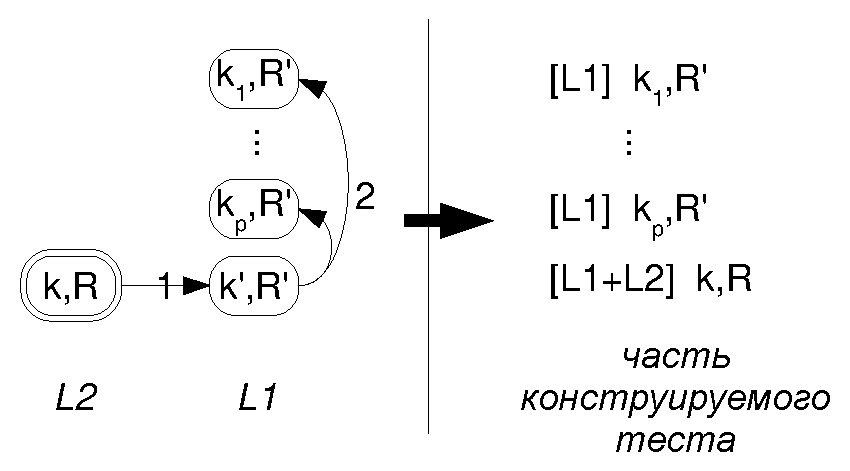
\includegraphics[width=0.6\textwidth]{2.theor/L1L2}
\caption{Конструирование обращения в кэш-память второго уровня вместе с
обращениями в кэш-память первого уровня}\label{fig:L1L2}
\end{figure}

Итак, по ключу и региону для кэш-памяти первого уровня
инструкция составляется по только что приведенной схеме. С одним лишь
уточнением, что адрес в этой инструкции должен быть таким, что при обращении по нему кэш-память
второго уровня не задействована. Теперь разберемся с последовательностью ключей
и регионов для кэш-памяти второго уровня. Рисунок~\ref{fig:L1L2} схематически
показывает, какие дополнительные инструкции надо построить для произвольного
обращения по ключу $k$ в регион $R$ кэш-памяти второго уровня. А именно, ключу
$k$ в регионе $R$ соответствует некоторый адрес, этому же адресу соответствуют и
некоторый ключ $k'$ в регионе $R'$ кэш-памяти первого уровня (стрелка с цифрой
1). Но надо еще обеспечить отсутствие этого ключа, иначе обращения в кэш-память
второго уровня не будет. Для этого надо сгенерировать небольшую
последовательность произвольных различных и не равных $k'$ ключей $k_1, k_2,
\dots, k_p$ и обратиться по ним в регион $R'$ кэш-памяти первого уровня без
затрагивания кэш-памяти второго уровня (значение числа $p$ зависит от стратегии
вытеснения).

%Рассмотрим один часто встречающийся случай кэширующих буферов,
%инициализация которого может вызывать трудности. Речь идет о
%кэш-памяти второго уровня. Зачастую кэш-память второго уровня не
%может быть инициализирована отдельно от остальных подсистем
%микропроцессора, обычно оно связано с изменением кэш-памяти первого
%уровня. Это создает дополнительные сложности при формулировании
%ограничений методом зеркальной генерации, поскольку инициализирующая
%последовательность должна подготавливать сразу два кэширующих буфера
%одновременно -- кэш-память первого уровня и кэш-память второго
%уровня. Кроме того, зачастую кэш-память второго уровня является
%совместной для хранения в ней данных и инструкций. Поэтому на
%инициализацию кэш-памяти второго уровня влияют и сами
%инициализирующие инструкции, и даже адрес расположения тестовой
%программы в памяти (от него зависит виртуальный адрес инструкций, а
%значит теги и индексы при обращении к кэш-памяти инструкций).
%
%Если принять дополнительное требование (и оно даст решение), что в
%кэш-памяти второго уровня наборы, используемые для доступа к
%инструкциям, не пересекаются с наборами, используемыми для доступа к
%данным, то генерируемые ограничения упрощаются (кэширование
%инструкций можно вообще не учитывать). С точки зрения зеркальной
%генерации это означает, что надо сформулировать требования на
%инициализирующую последовательность. Напомню, что одним из ключевых
%требований является произвольность начального состояния
%(содержимого) кэш-памяти.
%
%Предположим, что обращение к кэш-памяти второго уровня
%осуществляется при кэш-промахе в кэш-памяти первого уровня и
%кэш-память не является virtually indexed virtually
%tagged~\cite{HennessyPatterson3rd}. Для составления ограничений с
%использованием функций полезности необходимо знать, которые
%инструкции среди инициализирующей последовательности действительно
%обращаются в кэш-память второго уровня (иными словами, в каких
%инструкциях среди инициализирующей последовательности происходит
%кэш-промах при обращении к кэш-памяти первого уровня). Возможным
%решением было бы перебирать всевозможные распределения тестовых
%ситуаций в кэш-памяти первого уровня на элементах инициализирующей
%последовательности (с предварительной подготовкой этих тестовых
%ситуаций). Однако следующая лемма~\ref{special_initialization_L2}
%показывает, что для любого такого произвольного распределения
%тестовых ситуаций в кэш-памяти первого уровня существует решение со
%специальным распределением тестовых ситуаций. Это позволяет
%перебирать только такие специальные распределения тестовых ситуаций
%в кэш-памяти первого уровня. При этом вычислительная сложность
%процедуры поиска инициализирующей последовательности, дающей
%решение, изменяется от экспоненциальной от длины тестового шаблона к
%полиномиальной, что показывает лемма~\ref{max_k_h} (ее доказательство
%приведено в приложении~\ref{proofs}):
%\begin{lemma}[Верхняя оценка длины специальной инициализирующей
%последовательности для стратегии вытеснения \LRU]\label{max_k_h}\MaxUpperBoundLRU
%\end{lemma}
%\begin{sld}
%$$m = O(n)$$ где $m$ --- длина специальной инициализирующей
%последовательности, $n$ -- количество инструкций тестового шаблона.
%\end{sld}
%
%Для получения инициализирующей программы минимальной длины, можно
%применять сначала двоичный поиск суммы $k+h$ с применением
%дальнейшего поиска допустимых значений $k$ и $h$. 